
\documentclass[12pt,a4paper]{report}
  \usepackage[utf8]{inputenc}
  \usepackage[francais]{babel}
  \usepackage[T1]{fontenc}
  \usepackage{amsmath}
  \usepackage{amsfonts}
  \usepackage{amssymb}
  \usepackage{amsmath}
  \usepackage{textcomp}
  \usepackage{stmaryrd}
	\SetSymbolFont{stmry}{bold}{U}{stmry}{m}{n}
  \usepackage[Algorithme]{algorithm}
  \usepackage[center]{subfigure}
  \usepackage{algorithmic}
  \usepackage{placeins}
  %\usepackage{color}
 % \usepackage[hidelinks]{hyperref}
  \usepackage{minitoc} 
  
  %\RequirePackage{geometry}          % R\'egler la taille de la page
\RequirePackage{amsmath,amssymb,bm}% \'Etendre les fonctions maths
\RequirePackage{calc}              % Faire des calculs
\RequirePackage[centerlast,bf]{caption2} % Captions
\RequirePackage{array}             % Gestion des tableaux
\RequirePackage{tocbibind}         % ToC, ToF, etc. dans la ToC
\RequirePackage{ifpdf}             % Tester si g\'en\'eration d'un pdf

  \usepackage{fourier}
\usepackage{nota}
\usepackage{multirow}
\usepackage{breakcites}
%\usepackage[lined,boxed,french]{algorithm2e}
%\usepackage[ruled,vlined,french]{algorithm2e}

\ifpdf
   \RequirePackage[pdftex]{graphicx,color}
   \RequirePackage[pdftex,hidelinks]{hyperref}
%   \geometry{pdftex}
\else
   \RequirePackage[dvips]{graphicx,color}
   \RequirePackage[ps2pdf,hidelinks]{hyperref}
%   \geometry{dvips}
\fi

%\graphicspath{{figures/}}
 
\title{Bibliographie MECASIF - Extension de la PGD à des problèmes de dynamique non-linéaires}
\author{Pierre \bsc{Nargil}}
\date{28 avril 2014}

\begin{document}

\renewcommand{\thesection}{\arabic{section}} % remove the number of the chapter before the number of the section (avoid the zero).
\renewcommand{\contentsname}{Sommaire}
\renewcommand{\labelitemi}{$\bullet$}
\tableofcontents

\clearpage

\section{La PGD}
\subsection{Généralités}
La PGD, pour "Proper Generalized Decomposition", trouve son origine dans \cite{Lad85} sous le nom de "radial time-space approximation", comme faisant partie la méthode LATIN (voir également \cite{Lad89}). 

Parmi les possibilités apportées par la réduction de modèles, elle peut permettre de résoudre des problèmes jusque là inenvisageables, par exem\-ple dans la chimie quantique (quand des processus chimiques impliquent un nombre de molécules de réactifs si petit que le concept de continuité de concentration n'est plus valide, par exemple dans la recherche génétique). De tels problèmes peuvent rapidement être impossibles à résoudre par des méthodes standards, car ils souffrent de ce que l'on appelle la malédiction de la dimension. La solution est inaccessible par des approches traditionnelles de discrétisation utilisant un maillage car elles présentent une taille du système à résoudre qui croit exponentiellement en fonction du nombre de particules. Plus de détails sur ce sujet sont donnés dans \cite{Paradigm}.

La diminution drastique de temps de calcul apportée par la PGD permet d'envisager de nouvelles utilisations de la simulation, notamment dans les DDDAS (pour Dynamic Data-Driven Application System \cite{DDAS}), dont l'enjeu est de permettre à la simulation d'interagir avec une manipulation en temps réel. C'est-à-dire que les instruments actionneurs seront influencés par les résultats de calculs apportés par la simulation et les capteurs du système renverront des données à la simulation pour réajuster les calculs.

La PDG rencontre donc un franc succès depuis quelques années et ses applications sont pléthores. Un aperçu des différents travaux concernant cette méthode peut être trouvé dans \cite{ShortReview}.

Parmi les utilisations de la PGD on peut citer, l'application aux plaques dans \cite{bognet2012advanced}. La PGD est aussi utilisée dans le cadre de la dynamique dans \cite{boucinha2014ideal}. La méthode est étudiée également dans le cadre des problèmes inverses par \cite{louf2013fast,ghnatios2011methodological}


\subsection{Mise en place de nouvelles variables : nouvelles coordonnées}
La PGD présente un avantage, par la mise en place de coordonnées supplémentaires, comme le décrivent \cite{Paradigm} et \cite{DDAS}. Il s'agit de rajouter au produit de fonctions à variables séparées (à deux variables comme celui de la POD \cite{Chatterjee}), une fonction d'une nouvelle variable. Ceci permet de conserver une variable comme une inconnue et ainsi d'avoir un problème résolu quelque soit la valeur de cette variable. Pour obtenir un tel résultat sans cette méthode il faudrait effectuer de nombreux tirages de valeurs pour la variable et réaliser une approche de Monte Carlo, ce qui requerrait autant de résolutions. L'ajout de cette coordonnée permet donc de passer outre la nécessité de résoudre le problème pour chaque valeur d'une variable, et permet de résoudre une famille de problèmes qui dépendent de cette variable. C'est le principe de base de l'analyse stochastique, qui fait l'objet d'un intérêt grandissant. De cette manière la résolution du problème par la PGD apporte plus encore qu'une résolution directe, et peut permettre facilement la mise en place d'une optimisation. Ceci ne se limite pas à une valeur matériau et peut s'appliquer à une condition initiale ou à une valeur géométrique. 
Dans le cas de la valeur géométrique cela complexifie le problème et fait l'objet d'études en cours comme \cite{courard2013abaques,ammar2014parametric}.

%\subsection{Équations}
%Comme la POD, la PDG approxime la solution à l'aide de l'hypothèse de séparation des variables comme une somme de produits de fonctions; prenons la fonction solution $ z(x,t)$, elle sera approximée sous la forme :
%\begin{equation}
%z(x,t) \approx \sum^m_{k=1} a_k(t) \varphi_k(x)
%\end{equation}
%
%Mais à la différence de la POD, la fonction $z(x,t)$ est inconnue au préalable, on ne connaît alors pas les modes et on les calcule "à la volée", grâce à l'algorithme appelé algorithme des puissances itérées qui est le suivant :
%
%%\begin{center}
%%\begin{algorithm}
%%\KwData{this text}
%%\KwResult{how to write algorithm with \LaTeX2e }
%%initialization\;
%%\While{not at end of this document}{
%%read current\;
%%\eIf{understand}{
%%go to next section\;
%%current section becomes this one\;
%%}{
%%go back to the beginning of current section\;
%%}
%%}
%%\caption{How to write algorithms}
%%\end{algorithm}
%%\end{center}
%
%\begin{algorithm}
%\caption{Résolution PGD}
%\begin{algorithmic}[1]
%\FOR{$m = 1 $ à $ m_{max}$}
%\STATE initialiser $a_1$
%\FOR{$k = 1 $ à $ k_{max}$}
%\STATE $\varphi_k \leftarrow S_m(a_k )$
%\STATE normer $\varphi_k$ ($\Vert\varphi_k\Vert_\Omega = 1$)
%\STATE $a_k \leftarrow T_m (\varphi_k )$
%\STATE vérifier la convergence de $(\varphi_k a_k)$
%\ENDFOR
%\STATE $\varphi_m \leftarrow \varphi_k$ et $a_m \leftarrow a_k$
%\STATE $z_m = z_{m-1} + \varphi_m a_m$
%\ENDFOR
%\end{algorithmic}
%\label{AlgoPGD}
%\end{algorithm}
%\label{AlgoPGDPartie}
%
%%%%\REQUIRE $n \geq 0 \vee x \neq 0$
%%%%\ENSURE $y = x^n$
%%%\IF{$n < 0$}
%%%\STATE $N \leftarrow -n$
%%%\ELSE
%%%\STATE $N \leftarrow n$
%%%\ENDIF
%%%\STATE $N \leftarrow N - 1$
%%%\ENDFOR
%
%Où $\text{S}_m$ est l'application qui associe à une fonction du temps $a$, une fonction de l'espace $\varphi$. Et $\text{T}_m$ l'application qui associe à une fonction spatiale $\varphi$, une fonction temporelle $a$. On part de la formulation faible d'un problème :
%\begin{equation}
%\label{ProblemeLM}
%B(u,v) = L(v) ~~ \forall v \in H
%\end{equation}
%
%\label{LaxMilgram}
%\noindent
%Sous les hypothèses du théorème de Lax-Milgram :
%\begin{itemize}
%\item $H$ un espace de Hilbert
%\item $B$ un forme bilinéaire, continue et coercive sur $H$
%\item $L$ une forme linéaire continue sur $H$
%\end{itemize}
%il existe un unique u $\in$ H solution de l'équation \ref{ProblemeLM}.
%
%On applique alors la démarche classique pour la PGD, appelée Galerkin progressive. On suppose $z_{m-1}$ (l'approximation de $z$ à l'ordre $m-1$) connue. Un nouveau couple $(\varphi, a) \in  U \times V$ est défini pour la décomposition d'ordre $m$ comme celui qui vérifie le critère de double orthogonalité de Galerkin suivant:
%\begin{equation}
%\label{formulationFaible}
%B(z_{m-1} + \varphi a , \varphi a^* + \varphi^*  a) = L (\varphi a^* + \varphi^* a) ~~~
%\forall \varphi^*  \in U \text{ et } \forall a^* \in V 
%\end{equation}
%Alors $S_m (a)$ est définie par :
%\begin{equation}
%B(z_{m-1} + \varphi a , \varphi^*  a) = L (\varphi^* a) ~~~
%\forall \varphi^*  \in U
%\end{equation}
%et $T_m (\varphi)$ par :
%\begin{equation}
%B(z_{m-1} + \varphi a , \varphi a^*) = L (\varphi a^* ) ~~~
%\forall a^* \in V 
%\end{equation}
%
%Le couple $(\varphi, a)$ vérifie l'équation \ref{formulationFaible} si et seulement si $\varphi = S_m (a)$ et $a = T_m (\varphi)$, qui est un problème non-linéaire, dont la résolution par la PGD peut être vue comme un problème aux valeurs propres où $\varphi$ et $a$ sont respectivement les fonctions propres dominantes de $S_m \circ T_m$ et $T_m \circ S_m$ . Ce qui permet en s'inspirant d'algorithmes utilisés dans les problèmes aux valeurs propres d'obtenir l'algorithme 1, qui donne la décomposition. Cet algorithme peut être modifié, notamment par l'ajout de l'orthogonalisation qui peut généralement améliorer les résultats (dans le cas ou il n'y a que deux variables). S'il on veut orthogonaliser $\varphi_m$ par rapport à la base spatial existante \{$\varphi_1 , \varphi_2 , ... , \varphi_{m-1}$\}, il faut définir un produit scalaire sur $\Omega$, par exemple : 
%\begin{equation}
%\langle u,v \rangle_\Omega = \int_\Omega \! uv ~ d\Omega
%\end{equation}
%
%Une autre modification consiste à introduire une fonction $T(\mathbf{p_m}) = \boldsymbol{\alpha}_\mathbf{m}$, où $\mathbf{p_m}$ est un vecteur qui contient les $\varphi_m$, et $\boldsymbol{\alpha}_\mathbf{m}$ un vecteur contenant les $a_m$. Permettant ainsi la mise à jour de l'ensemble des fonctions du temps après chaque calcul d'un nouveau couple $(\varphi_m , a_m )$, 
%en remplaçant les lignes 9 et 10 de l'algorithme 1 par :
%
%\begin{algorithmic}
%\STATE $\varphi_m \leftarrow \varphi_k$
%\STATE $\boldsymbol{\alpha}_\mathbf{m} \leftarrow T(p_m)$
%\STATE $z_m = \mathbf{p_m} . \boldsymbol{\alpha}_\mathbf{m}$
%\end{algorithmic}
%
%Pour voir un exemple d'utilisation de la méthode, \cite{Garanteed} propose une résolution d'un problème thermique avec la PGD. Le calcul pour un problème dynamique sera détailler dans une autre partie.


\subsection{Équations avec paramètre}
Comme la POD, la PDG approxime la solution à l'aide de l'hypothèse de séparation des variables comme une somme de produits de fonctions; prenons la fonction solution $ z(x,t)$, elle sera approximée sous la forme :
\begin{equation}
z(x,t) \approx \sum^{m_{max}}_{m=1} \varphi_m(x) g_m(t) h_m(\theta)
\end{equation}

Mais à la différence de la POD, la fonction $z(x,t)$ est inconnue au préalable, on ne connaît alors pas les modes et on les calcule "à la volée".

On considère le problème :
\begin{equation}
\label{ProblemeLMPara}
B(u,v) = L(v) ~~ \forall v \in H
\end{equation}

\noindent
Sous les hypothèses du théorème de Lax-Milgram :
\begin{itemize}
\item $H$ un espace de Hilbert
\item $B$ un forme bilinéaire, continue et coercive sur $H$
\item $L$ une forme linéaire continue sur $H$
\end{itemize}
il existe un unique u $\in$ H solution de l'équation \ref{ProblemeLMPara}.

On applique alors la démarche classique pour la PGD, appelée Galerkin progressive. On suppose $z_{m-1}$ (l'approximation de $z$ à l'ordre $m-1$) connue. Un nouveau triplet $(\varphi, g, h) \in  U \times V \times W$ est défini pour la décomposition d'ordre $m$ comme celui qui vérifie le critère de double orthogonalité de Galerkin suivant:
\begin{equation}
\label{formulationFaiblePara}
\begin{array}{c}
B(z_{m-1} + \varphi g h , \varphi^*  g h + \varphi g^* h + \varphi g h^* ) = L (\varphi^*  g h + \varphi g^* h + \varphi g h^*) 
\\
\forall (\varphi, g, h) \in  U \times V \times W
\end{array}
\end{equation}
Alors $S^{\varphi}_m (g,h)$ est définie par :
\begin{equation}
B(z_{m-1} + \varphi g h , \varphi^*  g h) = L (\varphi^* g h) ~~~
\forall \varphi^*  \in U
\end{equation}
et $S^g_m (\varphi,h)$ par :
\begin{equation}
B(z_{m-1} + \varphi g h , \varphi  g^* h) = L (\varphi g^* h) ~~~
\forall g^* \in V 
\end{equation}

Le triplet $(\varphi, g, h)$ vérifie l'équation \ref{formulationFaiblePara} si et seulement si $\varphi = S^{\varphi}_m (g,h)$, $g = S^g_m (\varphi,h)$ et $ h = S^h_m (\varphi,g)$, qui est un problème non-linéaire. La résolution de celui-ci par la PGD peut être vue comme un problème aux valeurs propres.
% où $\varphi$, $g$ et $h$ sont respectivement les fonctions propres dominantes de $S^{\varphi}_m \circ S^g_m \circ S^h_m$, $S^g_m \circ S^h_m \circ S^{\varphi}_m$ et $S^h_m \circ S^{\varphi}_m \circ S^g_m$ . 
Ceci permet, en s'inspirant d'algorithmes utilisés dans les problèmes aux valeurs propres, d'obtenir l'algorithme \ref{AlgoPGDPara}, qui donne la décomposition en n-uplet. Cet algorithme peut être modifié, notamment par l'ajout de l'orthogonalisation qui peut généralement améliorer les résultats (dans le cas ou il n'y a que deux variables). L'orthogonalisation au delà de 2 variables séparées devient complexe et nécessite des travaux complémentaires..
\label{TrouverProblem}

% grâce à l'algorithme appelé algorithme des puissances itérées qui est le suivant :

\begin{algorithm}
\caption{Résolution PGD}
\begin{algorithmic}[1]
\FOR{$m = 1 $ à $ m_{max}$}
\STATE initialiser $a_1$
\FOR{$k = 1 $ à $ k_{max}$}
\STATE $\varphi_k \leftarrow S^{\varphi}_m(g_k,h_k)$
\STATE normer $\varphi_k$ ($\Vert\varphi_k\Vert_\Omega = 1$)
\STATE $g_k \leftarrow S^g_m (\varphi_k,h_k)$
\STATE normer $g_k$ ($\Vert g_k\Vert_T = 1$)
\STATE $h_k \leftarrow S^h_m (\varphi_k,g_k)$
\STATE vérifier la convergence de $(\varphi_k.g_k.g_k)$
\ENDFOR
\STATE $\varphi_m \leftarrow \varphi_k$, $g_m \leftarrow g_k$ et $h_m \leftarrow h_k$
\STATE $z_m = z_{m-1} + \varphi_m g_m h_m$
\ENDFOR
\end{algorithmic}
\label{AlgoPGDPara}
\end{algorithm}
\label{AlgoPGDPartiePara}

%%%\REQUIRE $n \geq 0 \vee x \neq 0$
%%%\ENSURE $y = x^n$
%%\IF{$n < 0$}
%%\STATE $N \leftarrow -n$
%%\ELSE
%%\STATE $N \leftarrow n$
%%\ENDIF
%%\STATE $N \leftarrow N - 1$
%%\ENDFOR

La méthode pour trouver les n-uplet de fonctions présentée ici est appelée Galerkin progressive, elle utilise un point fixe (boucle sur $k$ dans 
l'algorithme \ref{AlgoPGDPara}). Mais il existe d'autres méthodes, comme la minimisation du résidu. Une comparaison des méthodes est présentée dans \cite{nouy2010priori}, on peut noter que la minimisation apporte l'assurance de la convergence mais est plus couteuse en ressources de calcul.

----\cite{boucinha2013space}----
\FloatBarrier

\section{La méthode LATIN}

La méthode LATIN (Large Time INcrement method) \cite{Lad85,Lad99} a été initialement proposée pour traiter des problèmes non linéaires dépendants  du temps. Depuis son introduction, cette méthode a été exploitée autour de nombreux grands axes de développements :\\
\begin{itemize}
%\item Grandes déformations, plasticité (PGD)

\item Grandes transformations, formulation corotationnelle (PGD),
voir par exemple \cite{Boucard1997}

\item Elasto-visco-plasticité, grand nombre de cycles, thermo-élasto-visco-\\plasticité (PGD)
voir \cite{Cognard1999,pelle2000efficient}

\item Endommagement et composites,
voir \cite{Allix1992,Guinard2002,Saavedra-Redlich2012b}

\item Assemblages,
voir \cite{Lemoussu2000b,Champaney1996b}

\item Décomposition de domaine au sens large,
voir \cite{Loiseau2001,Ladeveze2002,Guidault2007,Violeau2006,Lad10}

\item Identification - Problèmes inverses,
voir \cite{Allix2002,Nguyen2008}

\item Multiparamétrique sans PGD,
voir \cite{Boucard03}

\item Multiparamétrique avec PGD,
voir \cite{Relun13}

\end{itemize}
  
\subsection{Notations}\label{not_latin}
% ----------------------------
Par simplicité est présenté ici un problème de thermique, avec $T$ la température et $\Ys$ le flux.
Pour simplifier l'écriture du problème, on introduit les espaces suivants (où $\bullet^*$ désigne les espaces homogènes associés) :\\
\begin{itemize}

\item L'espace $\CA$ des champs $T$ admissibles est comme précédemment :
 \begin{equation}
\mathcal{T} = \{ T \; | \quad T|_{ \bordT} = T_d \quad \textrm{et} \quad T|_{(t=0)} = \Tinit \}
\end{equation}

\item L'espace $\Ad$ des champs solution $(T, \Ys)$ admissibles :
 \begin{equation}
\Ad = \{ (T, \Ys) \; | \quad T \in \CA \quad \textrm{et} \quad  \diver{\Ys}+r = \mvol \capa \frac{\partial T}{\partial t} \quad \textrm{avec} \quad  \Ys  \cdot  \underline{n}|_{ \bordY } = y_d   \}
\end{equation}

\item L'espace $\Comp$ des champs solution $(T, \Ys)$ vérifiant la loi de Fourier :
 \begin{equation}
 \Comp = \left\{ (T, \Ys) \: | \: \underline{Y} = \conduc \:  \gradv{T} \right \}
\end{equation}

\end{itemize}


\subsection{Stratégie de résolution LATIN avec PGD}

On peut schématiser la méthode de résolution LATIN comme étant une stratégie qui génère une approximation de la solution $\mathbf{s}$ du problème sur l'ensemble de l'espace et du temps et en améliore automatiquement la qualité à chaque itération, quitte à commencer par une approximation très grossière. En ceci, la méthode est dite non incrémentale.
Cette méthode repose sur 3 principes de base ; la séparation des difficultés, l'approche itérative à 2 étapes et la représentation adaptée des inconnues.\\

%\begin{itemize}
%\item [$\blacktriangleright$] Le point P1 ou la séparation des difficultés \\
%\end {itemize}
  \paragraph{La séparation des difficultés }

Ce point consiste à traiter séparément les difficultés du problème en partitionnant l'espace constitué par l'ensemble des équations que le problème doit vérifier en 2 espaces distincts $\Comp$ et $\Ad$ comme définis en partie \ref{not_latin}. L'espace $\Comp$ est composé des champs vérifiant les équations locales, éventuellement non linéaires (par exemple, pour le problème de diffusion, si la conductivité $\conduc$ dépend de la température $T$), et l'espace $\Ad$ rassemble les champs vérifiant les équations linéaires éventuellement globales.
La solution du problème $\sols_{ref}=(T,\Ys)$ vérifie l'ensemble des équations et se trouve donc à l'intersection de ces 2 espaces : $\sols_{ref} = \Ad \cap \Comp$. (figure \ref{Latin_schema})

%\newpage
%\begin{itemize}
%\item [$\blacktriangleright$] Le point P2 ou l'approche itérative à 2 étapes \\
%\end {itemize}
  \paragraph{L'approche itérative à 2 étapes }

Pour trouver l'intersection de ces 2 espaces, on cherche alternativement une solution de l'un puis l'autre des espaces $\Comp$ et $\Ad$ : la stratégie est donc fondée sur une stratégie itérative à 2 étapes.\\ 


\begin{figure}[!htb]
\centering
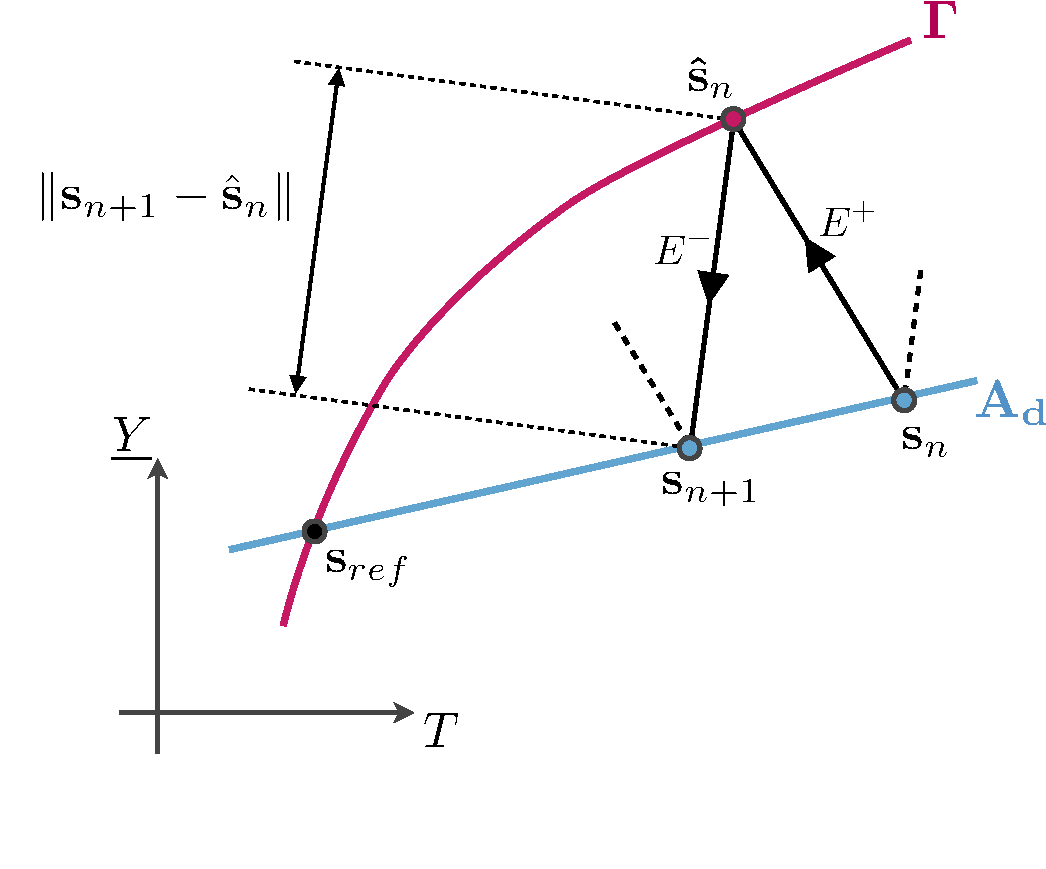
\includegraphics[width=8.8cm]{LATIN.figure/latin_iter_n1}
%\caption{Une itération à l'ordre $n+1$ de la méthode LATIN\label{fig:schema_rom_pgd}}
%\end{figure}
%\begin{figure}[!htb]
\begin{equation}
   \cdots\longrightarrow
   \sols_{n}\in\Ad
   \underbrace{
   \xrightarrow{\text{étape locale}}
   \solsc_{n}\in\Comp
   \xrightarrow{\text{étape linéaire}}
   \sols_{n+1}\in\Ad
   }_\text{iteration $n+1$}
   \longrightarrow
   \solsc_{n+1}
   \longrightarrow\cdots
\end{equation}
\caption{Une itération à l'ordre $n+1$ de la méthode LATIN\label{Latin_schema}}
\end{figure}


Il apparait sur le schéma de la figure \ref{Latin_schema} que l'on doit introduire des \og  directions de recherche\fg{} $\rechp$ et $\rechm$. En effet, le problème complet étant divisé en deux sous-problèmes complémentaires, chacun de ces sous-problèmes manque d'information. Les sous-problèmes n'ont donc pas d'unicité de la solution ou deviennent mal posés et on vient rajouter une équation par cette direction de recherche pour trouver une solution et qu'elle soit unique.\\
 On se donne les directions de recherche $\rechp$ pour l'étape locale et $\rechm$ pour l'étape linéaire (où $h$ est un paramètre de la méthode) :

\begin{equation}\label{dir_rech+}
\rechp:  \quad h\: (\hat{\Ys}_n-\Ys_n)+ (\gradv{\hat{T}_n}-\gradv{T_n}) = 0
\end{equation}
\begin{equation}\label{dir_rech-}
\rechm :  \quad h\: (\Ys_{n+1}-\hat{\Ys}_n)- (\gradv{T}_{n+1}-\gradv{\hat{T}}_n) = 0
\end{equation}\\


Comme schématisé sur la figure \ref{Latin_schema}, l'itération $n+1$ est donc composée :\\
\begin{itemize}
\item d'une étape locale, qui, partant d'une solution connue $\sols_{n} = (T_{n}, \Ys_{n}) \in \Ad$ cherche une solution $\solsc_{n} = (\hat{T}_{n}, \hat{\Ys}_{n}) \in \Comp$ en suivant la direction de recherche $E^+$, \\ 
\item d'une étape linéaire, qui, partant d'une solution connue $\solsc_{n} = (\hat{T}_{n}, \hat{\Ys}_{n}) \in \Comp$ cherche une solution $\sols_{n+1} = (T_{n+1}, \Ys_{n+1}) \in \Ad$ en suivant la direction de recherche $E^-$.\\
\end{itemize}


%\begin{itemize}
%\item [$\blacktriangleright$] Le point P3 ou la représentation adaptée des inconnues \\
%\end {itemize}
\paragraph{Réduction de modèles }

L'utilisation de la méthode LATIN autour des 2 seuls premiers points suffit à trouver la solution du problème. Cependant la convergence de la méthode est coûteuse avec cette architecture car la solution doit être améliorée à chaque itération sur l'ensemble de l'espace et du temps. En pratique, l'étape locale conduit à la résolution en chaque point d'espace d'un système différentiel en temps (généralement de petite taille) ce qui engendre un coût de calcul modique. En revanche, l'étape linéaire consiste à résoudre un problème global en espace pour chaque pas de temps.\\
La manipulation de la solution sur l'ensemble de l'espace et du temps est donc \textit{a priori} un inconvénient majeur pour le temps de calcul de la stratégie. Cependant, la connaissance de la solution sur $\inttps \times \domaine$ permet de mettre en œuvre les notions d'approximations spatio-temporelles qui vont en définitive permettre une grande réduction du temps de calcul. C'est donc avec ce troisième aspect que la méthode LATIN prend tout son sens.\\

La PGD permet de calculer l'approximation à variables séparées de la solution sans avoir besoin de réalisations. Elle doit donc être associée à une stratégie permettant de générer à la fois les fonctions du temps et les fonctions spatiales les plus pertinentes pour la solution. De plus, cette stratégie ne peut être incrémentale car chaque couple généré durant le processus doit améliorer l'approximation de la solution sur $\inttps \times \domaine$, ce qui est donc compatible avec la méthode LATIN.\\

Étant donné que le coût de l'étape locale est déjà réduit, on estime que l'introduction de la PGD au cours de cette étape ne constituera pas un réel gain et on choisit d'utiliser la représentation PGD uniquement durant l'étape linéaire.\\

L'ajout de la contrainte de représentation sous forme PGD des inconnues rend le problème, déjà constitué des 2 premiers points, sur-contraint. On ne pourra donc pas vérifier l'ensemble des équations. Le but étant ici de réduire le temps de calcul par l'utilisation de la PGD, on impose la représentation PGD des inconnues, et on ne peut ainsi jouer que sur les 2 premiers points de la méthode. Il apparait donc que 2 versions de la méthode LATIN avec PGD sont envisageables :\\

\begin{itemize}
\item Soit en vérifiant \og au mieux\fg{} la direction de recherche. La solution d'une étape s'obtiendra par la résolution d'un problème de minimisation sur l'écart entre la direction de recherche empruntée et celle voulue. On vérifiera donc exactement l'admissibilité de la solution et la représentation PGD. L'idée de cette version peut être schématisée par la figure \ref{rech_au_mieux}.\\
\item Soit en vérifiant \og au mieux\fg{} l'admissibilité de la solution à l'aide d'une approche Galerkin. On vérifiera donc exactement la direction de recher\-che et la représentation PGD. L'idée de cette version peut être schématisée par la figure \ref{ad_au_mieux}.\\
\end{itemize}
 
 
 
 \begin{figure}[!h]
\begin{center}
\begin{minipage}{5.7cm}
\begin{center}
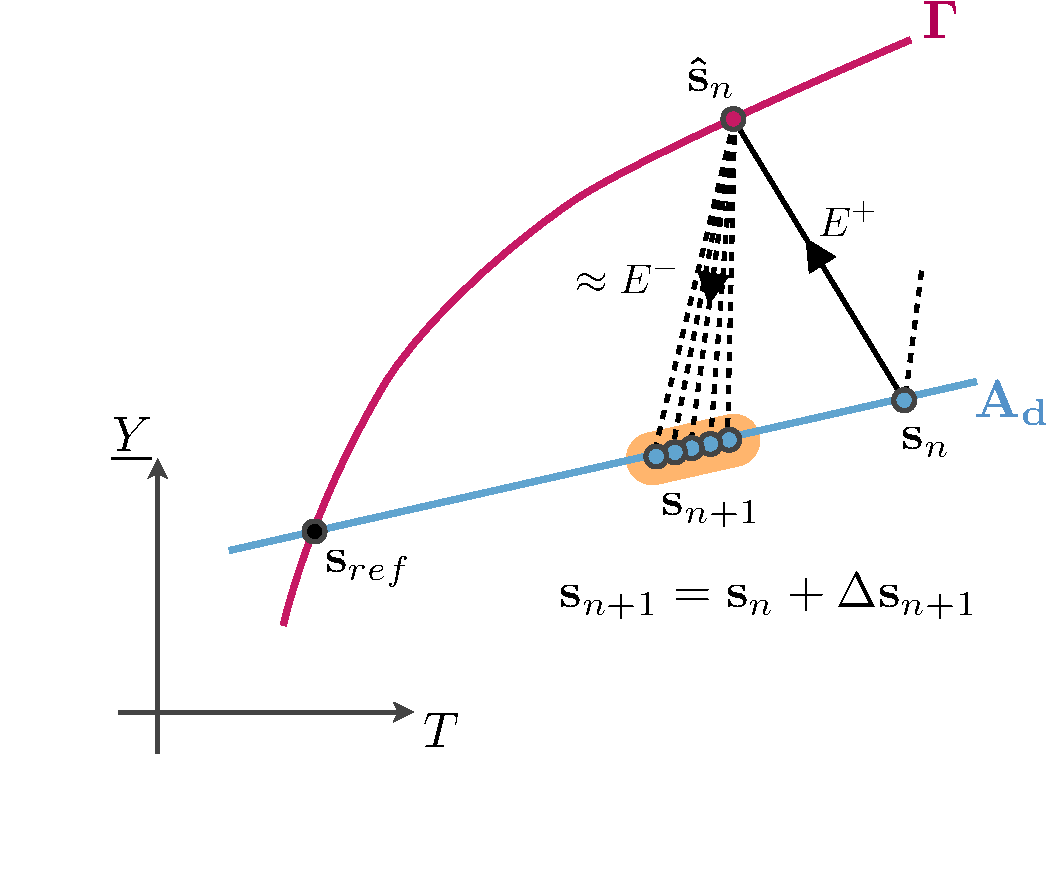
\includegraphics[height=5.45cm]{LATIN.figure/rech_au_mieux}\\
\caption{Vérification au mieux de la direction de recherche\label{rech_au_mieux}}
\end{center}
\end{minipage}%\hfill
\hspace{0.8cm}
\begin{minipage}{5.7cm}
\begin{center}
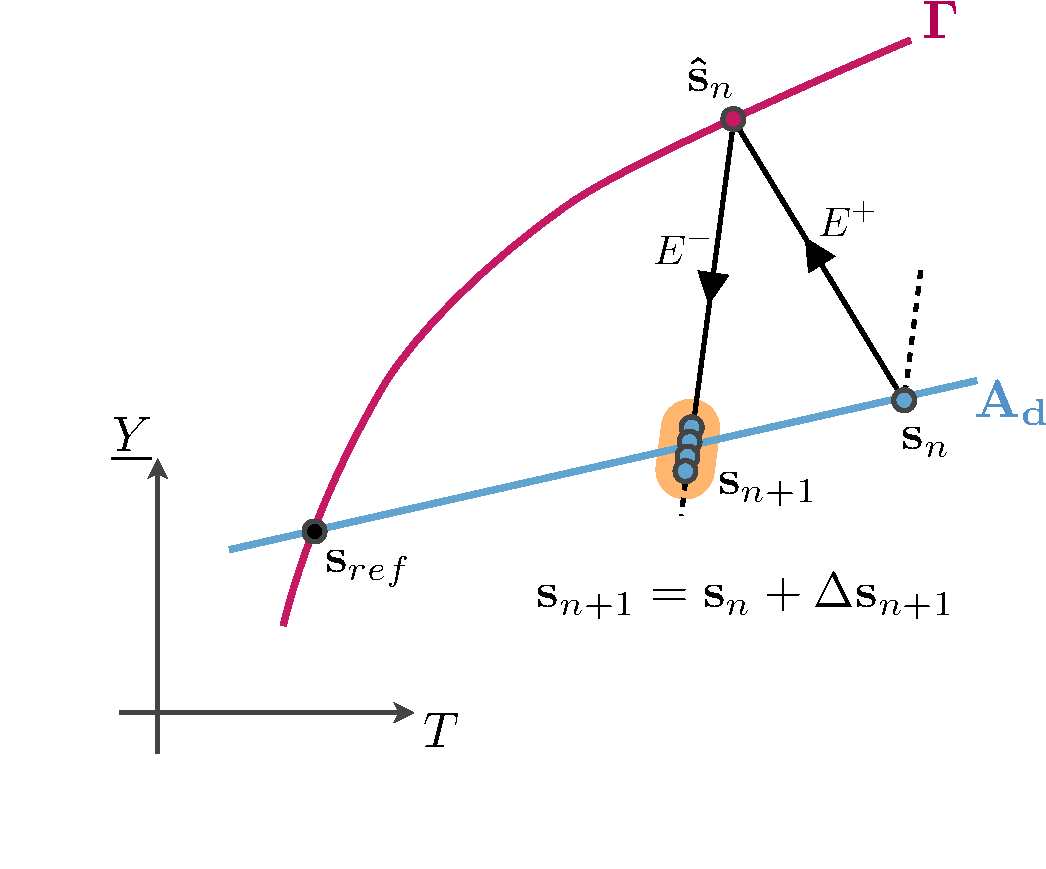
\includegraphics[height=5.45cm]{LATIN.figure/ad_au_mieux}\\
\caption{Admissibilité au mieux de $\sols_{n+1}$\label{ad_au_mieux}}
\end{center}
\end{minipage}
\end{center}
\end{figure}
 
 

 Pour des raisons de simplicité de mise en \oe{}uvre, on choisit de se placer dans le cadre d'une approche Galerkin. Ainsi, on vérifiera exactement la direction de recherche de la méthode ainsi que la représentation PGD de la solution, alors que la solution à chaque itération ne sera admissible qu'au mieux. Cette technique peut parfois mal converger mais ce n'est pas le cas pour le problème ici étudié \cite{Lad10}.\\ 
Etant donné que l'on vérifie exactement la direction de recherche \eqref{dir_rech-}, on peut toujours directement lier $\Ys$ à $T$. On peut donc toujours substituer la variable $\Ys$ par une expression ne dépendant que de $T$. La seule recherche de $T$ sous forme PGD est donc suffisante.\\
Durant l'itération $n+1$, on cherche à améliorer la solution $T_n \in \CA$ à l'aide d'un terme correctif $\Delta T_{n+1} \in \CA^*$. C'est cette correction qui est cherchée sous une forme à variables séparées. 
\begin{equation}
\begin{aligned}
T_{n+1}= T_n + \Delta T_{n+1} \quad \textrm{ où } \quad \Delta T_{n+1} = \tau_{n+1}(t) \: \mathbb{T}_{n+1} (\Ms)
\end{aligned}
\end{equation}


\section{La PGD en dynamique}

Dans le cadre du projet MECASIF, nous cherchons à appliquer la PGD à un problème de dynamique, voici le développement des équations.

\subsection{Définition du problème}

\begin{itemize}
\item Admissibilité cinématique :
	\\$U \in [H^1(\Omega)]^3, U_{|\partial \Omega_U} = U_d $
\item Admissibilité statique :
	\\$ div \sigma + f_v = \rho \ddot{U} + \mu \dot{U}$ sur $\Omega$ 
		et $\sigma . n _{|\partial \Omega_f} = f_d$
\item Relation de comportement :
	\\$\sigma = H : \varepsilon (U)$ sur $ \Omega$
\item Conditions initiales :
	\\$U(0) = U_0$ et $ \dot{U}(0) = \dot{U}_0$
\end{itemize}

\noindent
Formulation variationnelle : 
\begin{equation}
\begin{array}{l l}
	\forall U^* ~ \text{CA0,} & \displaystyle
		\int_\Omega [\varepsilon (U^*) : \sigma   
					+ U^* \mu \dot{U} 
					+ U^* \rho \ddot{U}
					- U^* f_d
					] d \Omega	
	\\& \displaystyle
		- \int_{\partial \Omega_f} U^* f_d  ds		
		- \underbrace{
			\int_{\partial \Omega_U} U^* \sigma . n ds	
		  }_{=0}
		= 0
\end{array}
\end{equation}

\noindent
Où
\begin{itemize}
\item $U$ est le déplacement
\item $\Omega$ l'espace, avec le bord $\partial \Omega = \partial \Omega_U \cap \partial \Omega_f$
\item $\sigma$ le tenseur des contraintes
\item $\varepsilon$ le tenseur des déformations
\item $\rho$ la masse volumique
\item $\mu$ l'amortissement volumique (mal connue)
\item $H$ le tenseur de Hooke
\item $f_v$ l'effort volumique
\item $f_d$ l'effort imposé sur $\partial \Omega_f$
\end{itemize}
\vspace{0.3cm}

\noindent
l'utilisation de l'hypothèse des variables séparables donne une expression de la forme :
\begin{equation}
	U(x,t,\theta) = \sum_{k=1}^n \varphi_k(x) g_k(t)h_k(\theta)
\end{equation}

\noindent
Où
\begin{itemize}
\item $x$ est la variable d'espace
\item $t$ la variable de temps
\item $\theta$ une variable paramètre (par exemple un module d'Young, un amortissement...)
\end{itemize}
\vspace{0.3cm}

Il faut discrétiser les fonctions sur leurs domaines de définition respectif. Ici la discrétisation en espace donne : 
\begin{equation}
	\begin{array}{l c l c l}
		\varphi(x) &=& \displaystyle \sum_{i=1}^{Nbc_x}  {N_\varphi}_i (x) \varphi_i &=& N_\varphi(x) \boldsymbol{\varphi_q} \\
	\end{array}
\end{equation}

$Nbc_x$ représente le nombre de composantes de discrétisation spatiale, l'indice $q$ représente le vecteur sur le domaine discrétisé.

On remplace dans la formulation variationnelle $U^*$ par 
\[  (\varphi gh)^* = ( \varphi^*gh+\varphi g^*h+\varphi gh^*) \]

\noindent
On rassemble les termes en $N_\varphi(x)$ ce qui permet de définir :
\begin{equation}
\mathbf{K} = \int_\Omega \varepsilon (N_\varphi(x)) : H : \varepsilon (N_\varphi(x))~~dx
\end{equation}
\begin{equation}
\mathbf{C} = \int_\Omega N_\varphi(x)^T \mu  N_\varphi(x)~~dx
\end{equation}
\begin{equation}
\mathbf{M} = \int_\Omega N_\varphi(x)^T \rho  N_\varphi(x)~~dx
\end{equation}
\begin{equation}
\mathbf{f} = \int_\Omega N_\varphi(x)^T f_v ~~dx 
	%+ \int_{\partial \Omega_U} U_d (H : \varepsilon (N_\varphi(x)) . n) 
	+ \int_{\partial \Omega_f} N_\varphi(x)^T f_d ~ds dt d\theta
\end{equation}

\noindent
Tous calculs fait cela donne :
\begin{equation}
\begin{array}{l l}
	\displaystyle	
	\int_T \! \int_\Theta	\!\!
		\big(\boldsymbol{\varphi_q}^*gh + \boldsymbol{\varphi_q}g^*h + \boldsymbol{\varphi_q}gh^*\big)^T \!
				&	\bigg[~\mathbf{K}~ \boldsymbol{\varphi_q}gh
						+ ~\mathbf{C}~ \boldsymbol{\varphi_q} \dot{g}h 
						+ ~\mathbf{M}~ \boldsymbol{\varphi_q} \ddot{g}h
	\\ 
	  &~~\displaystyle
			+ \mathbf{K} \sum_{k=1}^{n-1} (\boldsymbol{\varphi_q})_k       g_k  h_k 
			+ \mathbf{C} \sum_{k=1}^{n-1} (\boldsymbol{\varphi_q})_k  \dot{g_k} h_k 
	\\ &~~\displaystyle
			+ \mathbf{M} \sum_{k=1}^{n-1} (\boldsymbol{\varphi_q})_k \ddot{g_k} h_k
			 -\mathbf{f}~\bigg] ~dt d\theta
	= 0
\end{array}
\label{TotalProblem}
\end{equation}
Ce qui permet d'obtenir un problème à résoudre pour chaque variable, comme indiqué en \ref{TrouverProblem}

\subsection{Problème en espace}

On annule les termes en $g^*$ et $h^*$, pour obtenir :
\begin{equation}
\begin{array}{r r l}
	\forall \boldsymbol{\varphi_q}^*
	&\int_T \! \int_\Theta \!		\boldsymbol{\varphi_q}^{*T}gh &
						[~\mathbf{K}~ \boldsymbol{\varphi_q}gh
						+ ~\mathbf{C}~ \boldsymbol{\varphi_q} \dot{g}h 
						+ ~\mathbf{M}~ \boldsymbol{\varphi_q} \ddot{g}h
	\\ &&
			+ \mathbf{K}~ \sum_{k=1}^{n-1} (\boldsymbol{\varphi_q})_k       g_k  h_k 
			+  \mathbf{C}~ \sum_{k=1}^{n-1} (\boldsymbol{\varphi_q})_k  \dot{g_k} h_k 
	\\ && 
			+  \mathbf{M}~ \sum_{k=1}^{n-1} (\boldsymbol{\varphi_q})_k \ddot{g_k} h_k
			-\mathbf{f}~] ~dt d\theta ~~= 0
\end{array}
\end{equation}

\noindent
Donc:
\begin{equation}
\begin{array}{r l}
	\int_T \! \int_\Theta 	gh &
			[~\mathbf{K}~ \boldsymbol{\varphi_q}gh
			+ ~\mathbf{C}~ \boldsymbol{\varphi_q} \dot{g}h 
			+ ~\mathbf{M}~ \boldsymbol{\varphi_q} \ddot{g}h
	\\ &
			+ \mathbf{K}~ \sum_{k=1}^{n-1} (\boldsymbol{\varphi_q})_k       g_k  h_k 
			+  \mathbf{C}~ \sum_{k=1}^{n-1} (\boldsymbol{\varphi_q})_k  \dot{g_k} h_k 
	\\ &
			+  \mathbf{M}~ \sum_{k=1}^{n-1} (\boldsymbol{\varphi_q})_k \ddot{g_k} h_k
	  		- \mathbf{f}~] ~dt d\theta ~~= 0
\end{array}
\end{equation}

\noindent
Soit:
\begin{equation}
\begin{array}{l}
	-~ \displaystyle
		\int_T \! \int_\Theta
			gh [  ~\mathbf{K}~ gh
				+ ~\mathbf{C}~ \dot{g}h 
				+ ~\mathbf{M}~ \ddot{g}h
				] ~dt d\theta 
	~ \boldsymbol{\varphi_q}
	~~=
	\\
	\displaystyle
		\int_T \! \int_\Theta \!
			gh [  \mathbf{K} \! \sum_{k=1}^{n-1} (\boldsymbol{\varphi_q})_k       g_k  h_k 
				+ \mathbf{C} \! \sum_{k=1}^{n-1} (\boldsymbol{\varphi_q})_k  \dot{g_k} h_k 
				+ \mathbf{M} \! \sum_{k=1}^{n-1} (\boldsymbol{\varphi_q})_k \ddot{g_k} h_k
				- \mathbf{f}] ~dt d\theta				
\end{array}
\end{equation}
Ceci est un système auquel il faut rajouter les conditions limites en déplacement $U_d$ par une méthode adaptée : substitution, multiplicateurs de Lagrange... Dans le deuxième cas on change :

\begin{equation}
~\mathbf{M} \leftarrow
	\begin{bmatrix}
	   \mathbf{M} & 0 \\
	   0 & 0 \\
	\end{bmatrix}
	\textrm{,  }
	\mathbf{C} \leftarrow
	\begin{bmatrix}
	   \mathbf{C} & 0 \\
	   0 & 0 \\
	\end{bmatrix}
	\textrm{,  } 
	\mathbf{K} \leftarrow
	\begin{bmatrix}
	   \mathbf{K} & \mathbf{D}^T \\
	   \mathbf{D} & 0 \\
	\end{bmatrix}
	\textrm{,  }
	\boldsymbol{\varphi_q} \leftarrow
	\begin{bmatrix}
	   \boldsymbol{\varphi_q} \\
	   \boldsymbol{\lambda}\\
	\end{bmatrix}
	\textrm{ et }
	\mathbf{f} \leftarrow
	\begin{bmatrix}
	   \mathbf{f} \\
	   \mathbf{b} \\
	\end{bmatrix}
\end{equation}
où $\mathbf{D}$ et $\mathbf{b}$ représentent les déplacement imposés de la manière suivante:
\[ \mathbf{D} \boldsymbol{\varphi_q}= \mathbf{b} \]

\subsection{Problème en temps}

Partant de l'équation \ref{TotalProblem} on annule les termes en $\boldsymbol{\varphi_q}^*$ et $h^*$, pour obtenir :
\begin{equation}
\begin{array}{r r l}
	\forall g^*
	&\int_T \! \int_\Theta \!  \boldsymbol{\varphi_q}^Tg^*h &
						[~\mathbf{K}~ \boldsymbol{\varphi_q}gh
						+ ~\mathbf{C}~ \boldsymbol{\varphi_q} \dot{g}h 
						+ ~\mathbf{M}~ \boldsymbol{\varphi_q} \ddot{g}h
	\\ &&
			+ \mathbf{K}~ \sum_{k=1}^{n-1} (\boldsymbol{\varphi_q})_k       g_k  h_k 
			+  \mathbf{C}~ \sum_{k=1}^{n-1} (\boldsymbol{\varphi_q})_k  \dot{g_k} h_k 
	\\ &&
			+  \mathbf{M}~ \sum_{k=1}^{n-1} (\boldsymbol{\varphi_q})_k \ddot{g_k} h_k
			-\mathbf{f}~] ~dt d\theta ~~=0
\end{array}
\end{equation}

Donc:
\begin{equation}
\begin{array}{r l}
	\int_\Theta	\boldsymbol{\varphi_q}^Th &
				[  ~\mathbf{K}~ \boldsymbol{\varphi_q}gh
				+ ~\mathbf{C}~ \boldsymbol{\varphi_q}  \dot{g}h 
				+ ~\mathbf{M}~ \boldsymbol{\varphi_q} \ddot{g}h 
	\\ &
			+ \mathbf{K}~ \sum_{k=1}^{n-1} (\boldsymbol{\varphi_q})_k       g_k  h_k 
			+ ~\mathbf{C}~ \sum_{k=1}^{n-1} (\boldsymbol{\varphi_q})_k  \dot{g_k} h_k 
	\\ &
			+ ~\mathbf{M}~ \sum_{k=1}^{n-1} (\boldsymbol{\varphi_q})_k \ddot{g_k} h_k
			-\mathbf{f}~] ~d\theta ~~=0
\end{array}
\end{equation}

Soit:
\begin{equation}
\begin{array}{l}
	\displaystyle
		\int_\Theta	\!
			\boldsymbol{\varphi_q}^Th [    ~\mathbf{K}~ \boldsymbol{\varphi_q}h ] ~d\theta
	~g
	+ \!
		\int_\Theta	\!
			\boldsymbol{\varphi_q}^Th [ ~\mathbf{C}~ \boldsymbol{\varphi_q}h ] ~d\theta
	  ~\dot{g}
	+ \!
		\int_\Theta	\!
			\boldsymbol{\varphi_q}^Th [ ~\mathbf{M}~ \boldsymbol{\varphi_q}h ] ~d\theta
	  ~\ddot{g}
	  ~~ =
	\\
	- \! \displaystyle
		\int_\Theta		
			\boldsymbol{\varphi_q}^Th [  \mathbf{K}~ \sum_{k=1}^{n-1} (\boldsymbol{\varphi_q})_k       g_k  h_k 
				+ \mathbf{C} \sum_{k=1}^{n-1} (\boldsymbol{\varphi_q})_k  \dot{g_k} h_k 
				+ \mathbf{M} \sum_{k=1}^{n-1} (\boldsymbol{\varphi_q})_k \ddot{g_k} h_k
				- \mathbf{f} ] ~d\theta
\end{array}
\end{equation}

On se trouve donc en présence d'une équation différentielle en $g$, que l'on peut résoudre comme on résout classiquement un problème de dynamique, i.e. en utilisant un schéma d'intégration ou en utilisant des élément finis temporels.

\subsection{Problème en paramètre}

Partant de l'équation \ref{TotalProblem} on annule les termes en $\boldsymbol{\varphi_q}^*$ et $g^*$, pour obtenir :
  \begin{equation}
\begin{array}{r r l}
	\forall h^*
	&\int_T \! \int_\Theta \!  \boldsymbol{\varphi_q}^Tgh^* &
						[  ~\mathbf{K}~ \boldsymbol{\varphi_q}gh
						+ ~\mathbf{C}~ \boldsymbol{\varphi_q} \dot{g}h 
						+ ~\mathbf{M}~ \boldsymbol{\varphi_q} \ddot{g}h
	\\ &&
	  		+ \mathbf{K}~ \sum_{k=1}^{n-1} (\boldsymbol{\varphi_q})_k       g_k  h_k 
			+ \mathbf{C}~ \sum_{k=1}^{n-1} (\boldsymbol{\varphi_q})_k  \dot{g_k} h_k 
	\\ &&
			+ \mathbf{M}~ \sum_{k=1}^{n-1} (\boldsymbol{\varphi_q})_k \ddot{g_k} h_k
			-\mathbf{f}~] ~dt d\theta ~~=0
\end{array}
\end{equation}

On sort h (indépendant de $t$) de l'integrale sur $T$ :  
\begin{equation}
\begin{array}{r r l}
	\forall h^*
	&\int_\Theta \!  h^* \int_T \! g \boldsymbol{\varphi_q}^T &
						\left[  ~\mathbf{K}~ \boldsymbol{\varphi_q}g
							+ ~\mathbf{C}~ \boldsymbol{\varphi_q} \dot{g}
							+ ~\mathbf{M}~ \boldsymbol{\varphi_q} \ddot{g}
						\right]~dt ~ h ~d\theta
	\\ = &\int_\Theta \!  h^* \int_T \! g \boldsymbol{\varphi_q}^T &
	  		-[~ \mathbf{K}~ \sum_{k=1}^{n-1} (\boldsymbol{\varphi_q})_k       g_k  h_k 
			+ \mathbf{C}~ \sum_{k=1}^{n-1} (\boldsymbol{\varphi_q})_k  \dot{g_k} h_k 
	\\ &&
			+ \mathbf{M}~ \sum_{k=1}^{n-1} (\boldsymbol{\varphi_q})_k \ddot{g_k} h_k
			-\mathbf{f}~] ~dt d\theta 
\end{array}
\end{equation}

Contrairement au problème précédant (en temps) on a une dépendance des termes intégrés par rapport à la variable $\theta$. Pour continuer on fait donc apparaitre la forme discrétisée :
\begin{equation}
	\begin{array}{l c l c l}
		h(\theta) &=& \displaystyle \sum_{i=1}^{Nbc_\theta}  {N_h}_i (\theta) h_i &=& N_h(\theta) \boldsymbol{h_q} \\
	\end{array}
\end{equation}

Ce qui donne :
\begin{equation}
\begin{array}{r r l}
	\forall \boldsymbol{h_q}^*
	&\int_\Theta \!  \boldsymbol{h_q}^{*T} N_h(\theta)^{T}  \!\! \int_T \! g \boldsymbol{\varphi_q}^T &
						\left[  \mathbf{K} \boldsymbol{\varphi_q}g
							+ \mathbf{C} \boldsymbol{\varphi_q} \dot{g}
							+ \mathbf{M} \boldsymbol{\varphi_q} \ddot{g}
						\right] dt  N_h(\theta) \boldsymbol{h_q} d\theta
	\\ = &\int_\Theta \!  \boldsymbol{h_q}^{*T} N_h(\theta)^{T}  \!\! \int_T \! g \boldsymbol{\varphi_q}^T &
	  		-[~ \mathbf{K}~ \sum_{k=1}^{n-1} (\boldsymbol{\varphi_q})_k       g_k N_h(\theta) (\boldsymbol{h_q})_k 
	  \\&& \phantom{-[}
			+ \mathbf{C}~ \sum_{k=1}^{n-1} (\boldsymbol{\varphi_q})_k  \dot{g_k} N_h(\theta) (\boldsymbol{h_q})_k 
	  \\&& \phantom{-[}
			+ \mathbf{M}~ \sum_{k=1}^{n-1} (\boldsymbol{\varphi_q})_k \ddot{g_k} N_h(\theta) (\boldsymbol{h_q})_k
	  \\&& \phantom{-[}
			-\mathbf{f}~] ~dt d\theta 
\end{array}
\end{equation}

Donc :
\begin{equation}
\begin{array}{r r l}
	&\int_\Theta \!  N_h(\theta)^{T}  \!\! \int_T \! g \boldsymbol{\varphi_q}^T &
						\left[  \mathbf{K} \boldsymbol{\varphi_q}g
							+ \mathbf{C} \boldsymbol{\varphi_q} \dot{g}
							+ \mathbf{M} \boldsymbol{\varphi_q} \ddot{g}
						\right] dt  N_h(\theta) \boldsymbol{h_q} d\theta
	\\ = &\int_\Theta \!  N_h(\theta)^{T}  \!\! \int_T \! g \boldsymbol{\varphi_q}^T &
	  		-[~ \mathbf{K}~ \sum_{k=1}^{n-1} (\boldsymbol{\varphi_q})_k       g_k N_h(\theta) (\boldsymbol{h_q})_k 
	  \\&& \phantom{-[}
			+ \mathbf{C}~ \sum_{k=1}^{n-1} (\boldsymbol{\varphi_q})_k  \dot{g_k} N_h(\theta) (\boldsymbol{h_q})_k 
	  \\&& \phantom{-[}
			+ \mathbf{M}~ \sum_{k=1}^{n-1} (\boldsymbol{\varphi_q})_k \ddot{g_k} N_h(\theta) (\boldsymbol{h_q})_k
	  \\&& \phantom{-[}
			-\mathbf{f}~] ~dt d\theta 
\end{array}
\end{equation}
  
On sort l'inconnue $\boldsymbol{h_q}$ pour obtenir le système:
\begin{equation}
\begin{array}{r r l}
	&\int_\Theta \!  N_h(\theta)^{T}  \!\! \int_T \! g \boldsymbol{\varphi_q}^T &
						\left[  \mathbf{K} \boldsymbol{\varphi_q}g
							+ \mathbf{C} \boldsymbol{\varphi_q} \dot{g}
							+ \mathbf{M} \boldsymbol{\varphi_q} \ddot{g}
						\right] dt  N_h(\theta) d\theta \boldsymbol{h_q}
	\\ = &\int_\Theta \!  N_h(\theta)^{T}  \!\! \int_T \! g \boldsymbol{\varphi_q}^T &
	  		-[~ \mathbf{K}~ \sum_{k=1}^{n-1} (\boldsymbol{\varphi_q})_k       g_k N_h(\theta) (\boldsymbol{h_q})_k 
	  \\&& \phantom{-[}
			+ \mathbf{C}~ \sum_{k=1}^{n-1} (\boldsymbol{\varphi_q})_k  \dot{g_k} N_h(\theta) (\boldsymbol{h_q})_k 
	  \\&& \phantom{-[}
			+ \mathbf{M}~ \sum_{k=1}^{n-1} (\boldsymbol{\varphi_q})_k \ddot{g_k} N_h(\theta) (\boldsymbol{h_q})_k
	  \\&& \phantom{-[}
			-\mathbf{f}~] ~dt d\theta 
\end{array}
\end{equation}

Et pour continuer les calculs il faudrait expliciter la dépendance des termes par rapport à $\theta$.

\newpage


\addcontentsline{toc}{part}{Bibliographie} 
\bibliographystyle{ieeetr}
\bibliography{Biblio}

%\newpage
%
%\appendix
%
%
%\section{Calcul du problème PGD étape par étape}
%%\documentclass[10pt]{report}
%
%\begin{document}
\begin{itemize}
\item Admissibilité cinématique :
	\\$U \in [H^1(\Omega)]^3, U_{|\partial \Omega_U} = U_d $
\item Admissibilité statique :
	\\$ div \sigma + f_v = \rho \ddot{U} + \mu \dot{U}$ sur $\Omega$ 
		et $\sigma . n _{|\partial \Omega_f} = f_d$
\item Relation de comportement :
	\\$\sigma = H : \epsilon (U)$ sur $ \Omega$
\item Conditions initiales :
	\\$U(0) = U_0$ et $ \dot{U}(0) = \dot{U}_0$
\end{itemize}

\noindent
Formulation variationnelle : 
\begin{equation}
	\forall U^* ~ \text{CA0,} ~
		\int_\Omega [\epsilon (U^*) : \sigma   
					+ U^* \mu \dot{U} 
					+ U^* \rho \ddot{U}
					- U^* f_d
					] d \Omega	
		- \int_{\partial \Omega_f} U^* f_d  ds		
		- \underbrace{
			\int_{\partial \Omega_U} U^* \sigma . n ds	
		  }_{=0}
		= 0
\end{equation}

\noindent
Où
\begin{itemize}
\item $U$ est le déplacement
\item $\Omega$ l'espace, avec le bord $\partial \Omega = \partial \Omega_U \cap \partial \Omega_f$
\item $\sigma$ le tenseur des contraintes
\item $\epsilon$ le tenseur des déformations
\item $\rho$ la masse volumique
\item $\mu$ expression de la viscosité (cette donnée est généralement mal connue)
\item $H$ le tenseur de Hook
\item $f_v$ effort volumique
\item $f_d$ effort imposé que le bord de $\Omega$
\end{itemize}
\vspace{0.3cm}

\noindent
Mise en place de la PGD, utilisation de l'hypothèse des variables séparables :
\begin{equation}
	U(x,t,\theta) = \sum_{k=1}^n \phi_k(x) g_k(t)h_k(\theta)
\end{equation}

Pour chaque $k$, il faut discrétiser les fonctions sur leur domaine de définition : 
\begin{equation}
	\begin{array}{l c l c l}
		\phi(x) &=& \sum_{i=1}^{Nbc_x}  N_i (x) \phi_i &=& N_\phi(x) \boldsymbol{\phi_q}
		\\
		g(t) &=& \sum_{i=1}^{Nbc_t}  N_i (t) gi &=& N_g(t) \mathbf{g_q}
		\\
		h(\theta) &=& \sum_{i=1}^{Nbc_\theta}  N_i (\theta) hi 
		&=& N_h(\theta) \mathbf{h_q}
	\end{array}
\end{equation}
$Nbc_x$ Représente le nombre de composante de discrétisation spatiale, l'indice $q$ représente le vecteur sur le domaine discrétisé.
\\
On remplace dans la formulation variationnelle, en choisissant $U^* = (\phi gh)^* = ( \phi^*gh+\phi g^*h+\phi gh^*) $ :
\begin{equation}
\begin{array}{r r l}
	&\int_\Omega \! \int_T \! \int_\Theta \!\!\!&		
		[\epsilon (\phi^*gh) : H : \epsilon (U_n)
			+ \phi^*gh \mu \dot{U_n} 
			+ \phi^*gh \rho \ddot{U_n}
			- \phi^*gh f_v
			] ~dx dt d\theta
	\\
	+ &\int_\Omega \! \int_T \! \int_\Theta \!\!\!&		
		[\epsilon (\phi g^*h) : H : \epsilon (U_n)
			+ \phi g^*h \mu \dot{U_n} 
			+ \phi g^*h \rho \ddot{U_n}
			- \phi g^*h f_v
			] ~dx dt d\theta
	\\
	+ &\int_\Omega \! \int_T \! \int_\Theta \!\!\!&		
		[\epsilon (\phi gh^*) : H : \epsilon (U_n)
			+ \phi gh^* \mu \dot{U_n} 
			+ \phi gh^* \rho \ddot{U_n}
			- \phi gh^* f_v
			] ~dx dt d\theta
	\\
	- &\int_{\partial \Omega_\mathbf{f}} \! \int_T \! \int_\Theta \!\!\!&
		(\phi^*gh + \phi g^*h + \phi gh^*) f_d  ~ds dt d\theta
\\
	= &0& 
\end{array}
\end{equation}

Puis $U = U_{n} = U_{n-1} + \phi gh$ :
\begin{equation}
\begin{array}{r r l}
	&\int_\Omega \! \int_T \! \int_\Theta \!\!\!&		
		gh[\epsilon (\phi^*) : H : \epsilon (U_{n-1} + \phi gh)
			+ \phi^* \mu \dot{(U_{n-1} + \phi gh)} 
			+ \phi^* \rho \ddot{(U_{n-1} + \phi gh)}
			- \phi^* f_v
			] ~dx dt d\theta
	\\
	+ &\int_\Omega \! \int_T \! \int_\Theta \!\!\!&		
		g^*h[\epsilon (\phi) : H : \epsilon (U_{n-1} + \phi gh)
			+ \phi \mu \dot{(U_{n-1} + \phi gh)} 
			+ \phi \rho \ddot{(U_{n-1} + \phi gh)}
			- \phi f_v
			] ~dx dt d\theta
	\\
	+ &\int_\Omega \! \int_T \! \int_\Theta \!\!\!&		
		gh^*[\epsilon (\phi) : H : \epsilon (U_{n-1} + \phi gh)
			+ \phi \mu \dot{(U_{n-1} + \phi gh)} 
			+ \phi \rho \ddot{(U_{n-1} + \phi gh)}
			- \phi f_v
			] ~dx dt d\theta
	\\
	- &\int_{\partial \Omega_\mathbf{f}} \! \int_T \! \int_\Theta \!\!\!&
		(\phi^*gh + \phi g^*h + \phi gh^*) f_d  ~ds dt d\theta
\\
	= &0& 
\end{array}
\end{equation}

On distribue la dérivation : 
\begin{equation}
\begin{array}{r r l}
	&\int_\Omega \! \int_T \! \int_\Theta \!\!\!&		
		gh[\epsilon (\phi^*) : H : \epsilon (U_{n-1} + \phi gh)
			+ \phi^* \mu (\dot{U_{n-1}} + \phi \dot{g}h)
			+ \phi^* \rho (\ddot{U_{n-1}} + \phi \ddot{g}h)
			- \phi^* f_v
			] ~dx dt d\theta
	\\
	+ &\int_\Omega \! \int_T \! \int_\Theta \!\!\!&		
		g^*h[\epsilon (\phi) : H : \epsilon (U_{n-1} + \phi gh)
			+ \phi \mu (\dot{U_{n-1}} + \phi \dot{g}h) 
			+ \phi \rho (\ddot{U_{n-1}} + \phi \ddot{g}h)
			- \phi f_v
			] ~dx dt d\theta
	\\
	+ &\int_\Omega \! \int_T \! \int_\Theta \!\!\!&		
		gh^*[\epsilon (\phi) : H : \epsilon (U_{n-1} + \phi gh)
			+ \phi \mu (\dot{U_{n-1}} + \phi\dot{g}h)
			+ \phi \rho (\ddot{U_{n-1}} + \phi\ddot{g}h)
			- \phi f_v
			] ~dx dt d\theta
	\\
	- &\int_{\partial \Omega_\mathbf{f}} \! \int_T \! \int_\Theta \!\!\!&
		(\phi^*gh + \phi g^*h + \phi gh^*) f_d  ~ds dt d\theta
\\
	= &0& 
\end{array}
\end{equation}

On sépare les termes en $n-1$ des termes virtuels :
\begin{equation}
\begin{array}{r r l}
	&\int_\Omega \! \int_T \! \int_\Theta \!\!\!&		
		gh[\epsilon (\phi^*) : H : \epsilon (\phi gh)
			+ \phi^* \mu \phi\dot{g}h
			+ \phi^* \rho \phi\ddot{g}h
			- \phi^* f_v
			] ~dx dt d\theta
	\\
	+ &\int_\Omega \! \int_T \! \int_\Theta \!\!\!&		
		gh[\epsilon (\phi^*) : H : \epsilon (U_{n-1})
			+ \phi^* \mu \dot{U_{n-1}} 
			+ \phi^* \rho \ddot{U_{n-1}}
			] ~dx dt d\theta
	\\
	+ &\int_\Omega \! \int_T \! \int_\Theta \!\!\!&		
		g^*h[\epsilon (\phi) : H : \epsilon ( \phi gh)
			+ \phi \mu  \phi\dot{g}h
			+ \phi \rho \phi\ddot{g}h
			- \phi f_v
			] ~dx dt d\theta
	\\
	+ &\int_\Omega \! \int_T \! \int_\Theta \!\!\!&		
		g^*h[\epsilon (\phi) : H : \epsilon (U_{n-1})
			+ \phi \mu \dot{U_{n-1}}
			+ \phi \rho \ddot{U_{n-1}}
			] ~dx dt d\theta
	\\
	+ &\int_\Omega \! \int_T \! \int_\Theta \!\!\!&		
		gh^*[\epsilon (\phi) : H : \epsilon (\phi gh)
			+ \phi \mu + \phi\dot{g}h
			+ \phi \rho \phi\ddot{g}h
			- \phi f_v
			] ~dx dt d\theta
	\\
	+ &\int_\Omega \! \int_T \! \int_\Theta \!\!\!&		
		gh^*[\epsilon (\phi) : H : \epsilon (U_{n-1})
			+ \phi \mu \dot{U_{n-1}}
			+ \phi \rho \ddot{U_{n-1}}
			- \phi f_v
			] ~dx dt d\theta
	\\
	- &\int_{\partial \Omega_\mathbf{f}} \! \int_T \! \int_\Theta \!\!\!&
		(\phi^*gh + \phi g^*h + \phi gh^*) f_d  ~ds dt d\theta
	\\
	= &0& 
\end{array}
\end{equation}

On peut regrouper les termes qui n'ont pas de partie virtuel en espace i.e. $\phi^*$ :
\begin{equation}
\begin{array}{r r l}
	&\int_\Omega \! \int_T \! \int_\Theta \!\!\!&		
		gh[\epsilon (\phi^*) : H : \epsilon (\phi gh)
			+ \phi^* \mu \phi\dot{g}h
			+ \phi^* \rho \phi\ddot{g}h
			- \phi^* f_v
			] ~dx dt d\theta
	\\
	+ &\int_\Omega \! \int_T \! \int_\Theta \!\!\!&		
		gh[\epsilon (\phi^*) : H : \epsilon (U_{n-1})
			+ \phi^* \mu \dot{U_{n-1}} 
			+ \phi^* \rho \ddot{U_{n-1}}
			] ~dx dt d\theta
	\\
	+ &\int_\Omega \! \int_T \! \int_\Theta \!\!\!&		
		(g^*h + gh^*)[\epsilon (\phi) : H : \epsilon ( \phi gh)
			+ \phi \mu  \phi\dot{g}h
			+ \phi \rho \phi\ddot{g}h
			- \phi f_v
			] ~dx dt d\theta
	\\
	+ &\int_\Omega \! \int_T \! \int_\Theta \!\!\!&		
		(g^*h + gh^*)[\epsilon (\phi) : H : \epsilon (U_{n-1})
			+ \phi \mu \dot{U_{n-1}}
			+ \phi \rho \ddot{U_{n-1}}
			] ~dx dt d\theta
	\\
	- &\int_{\partial \Omega_\mathbf{f}} \! \int_T \! \int_\Theta \!\!\!&
		(\phi^*gh + \phi g^*h + \phi gh^*) f_d  ~ds dt d\theta
	\\
	= &0& 
\end{array}
\end{equation}

On discrétise en espace :
\begin{equation}
\begin{array}{r r l}
	&\int_\Omega \! \int_T \! \int_\Theta \!\!\!&		
		gh\boldsymbol{\phi_q}^*[\epsilon (N_\phi(x)) : H : \epsilon (N_\phi(x)\boldsymbol{\phi_q} gh)
			+ N_\phi(x) \mu  N_\phi(x) \boldsymbol{\phi_q}  \dot{g}h
			\\ && \phantom{gh\boldsymbol{\phi_q}^*[ }
			+ N_\phi(x) \rho N_\phi(x) \boldsymbol{\phi_q} \ddot{g}h
			- N_\phi(x) f_v
			] ~dx dt d\theta
	\\
	+ &\int_\Omega \! \int_T \! \int_\Theta \!\!\!&		
		gh\boldsymbol{\phi_q}^*[\epsilon (N_\phi(x)) : H : \epsilon (U_{n-1})
			+ N_\phi(x) \mu \dot{U_{n-1}} 
			+ N_\phi(x) \rho \ddot{U_{n-1}}
			] ~dx dt d\theta
	\\
	+ &\int_\Omega \! \int_T \! \int_\Theta \!\!\!&		
		(g^*h + gh^*)\boldsymbol{\phi_q}[\epsilon (N_\phi(x)) : H : \epsilon (N_\phi(x) \boldsymbol{\phi_q}gh)
			+ N_\phi(x) \mu  N_\phi(x) \boldsymbol{\phi_q} \dot{g}h
			\\ && \phantom{(g^*h + gh^*)\boldsymbol{\phi_q}[ }
			 + N_\phi(x) \rho N_\phi(x) \boldsymbol{\phi_q} \ddot{g}h
			- N_\phi(x) f_v
			] ~dx dt d\theta
	\\
	+ &\int_\Omega \! \int_T \! \int_\Theta \!\!\!&		
		(g^*h + gh^*)\boldsymbol{\phi_q}[\epsilon (N_\phi(x)) : H : \epsilon (U_{n-1})
			+ N_\phi(x) \mu \dot{U_{n-1}}
			+ N_\phi(x) \rho \ddot{U_{n-1}}
			] ~dx dt d\theta
	\\
	- &\int_{\partial \Omega_\mathbf{f}} \! \int_T \! \int_\Theta \!\!\!&
		N_\phi(x)(\boldsymbol{\phi_q}^*gh + \boldsymbol{\phi_q} g^*h + \boldsymbol{\phi_q} gh^*) f_d  ~ds dt d\theta
	\\
	= &0& 
\end{array}
\end{equation}

\begin{equation}
U_{n-1}(x,t,\theta)
	 = \sum_{k=1}^{n-1} \phi_k(x) g_k(t)h_k(\theta)
	 = \sum_{k=1}^{n-1} N_\phi(x)(\boldsymbol{\phi_q})_k g_k(t)h_k(\theta)
\end{equation}

En utilisant la formule précédente :
\begin{equation}
\begin{array}{r r l}
	&\int_\Omega \! \int_T \! \int_\Theta \!\!\!&		
		gh\boldsymbol{\phi_q}^*[\epsilon (N_\phi(x)) : H : \epsilon (N_\phi(x)\boldsymbol{\phi_q} gh)
			\\ && \phantom{gh\boldsymbol{\phi_q}^*[ }
			+ N_\phi(x) \mu  N_\phi(x) \boldsymbol{\phi_q}  \dot{g}h
			\\ && \phantom{gh\boldsymbol{\phi_q}^*[ }
			+ N_\phi(x) \rho N_\phi(x) \boldsymbol{\phi_q} \ddot{g}h
			- N_\phi(x) f_v
			] ~dx dt d\theta
	\\
	+ &\int_\Omega \! \int_T \! \int_\Theta \!\!\!&		
		gh\boldsymbol{\phi_q}^*[\epsilon (N_\phi(x)) : H : 
				\epsilon (\sum_{k=1}^{n-1} N_\phi(x)(\boldsymbol{\phi_q})_k g_k h_k)
			\\ && \phantom{gh\boldsymbol{\phi_q}^*[}
			+ N_\phi(x) \mu \sum_{k=1}^{n-1} N_\phi(x)(\boldsymbol{\phi_q})_k \dot{g_k} h_k 
			\\ && \phantom{gh\boldsymbol{\phi_q}^*[}
			+ N_\phi(x) \rho \sum_{k=1}^{n-1} N_\phi(x)(\boldsymbol{\phi_q})_k \ddot{g_k} h_k 
			] ~dx dt d\theta
	\\
	+ &\int_\Omega \! \int_T \! \int_\Theta \!\!\!&		
		(g^*h + gh^*)\boldsymbol{\phi_q}[\epsilon (N_\phi(x)) : H : \epsilon (N_\phi(x) \boldsymbol{\phi_q}gh)
			\\ && \phantom{(g^*h + gh^*)\boldsymbol{\phi_q}[ }
			+ N_\phi(x) \mu  N_\phi(x) \boldsymbol{\phi_q} \dot{g}h
			\\ && \phantom{(g^*h + gh^*)\boldsymbol{\phi_q}[ }
			 + N_\phi(x) \rho N_\phi(x) \boldsymbol{\phi_q} \ddot{g}h
			- N_\phi(x) f_v
			] ~dx dt d\theta
	\\
	+ &\int_\Omega \! \int_T \! \int_\Theta \!\!\!&
		(g^*h + gh^*)\boldsymbol{\phi_q}[\epsilon (N_\phi(x)) : H : 
					\epsilon (\sum_{k=1}^{n-1} N_\phi(x)(\boldsymbol{\phi_q})_k \dot{g_k} h_k )
			\\ && \phantom{(g^*h + gh^*)\boldsymbol{\phi_q}[}
			+ N_\phi(x) \mu \sum_{k=1}^{n-1} N_\phi(x)(\boldsymbol{\phi_q})_k \dot{g_k} h_k 
			\\ && \phantom{(g^*h + gh^*)\boldsymbol{\phi_q}[}
			+ N_\phi(x) \rho \sum_{k=1}^{n-1} N_\phi(x)(\boldsymbol{\phi_q})_k \ddot{g_k} h_k 
			] ~dx dt d\theta
	\\
	- &\int_{\partial \Omega_\mathbf{f}} \! \int_T \! \int_\Theta \!\!\!&
		N_\phi(x)(\boldsymbol{\phi_q}^*gh + \boldsymbol{\phi_q} g^*h + \boldsymbol{\phi_q} gh^*) f_d  ~ds dt d\theta
	\\
	= &0& 
\end{array}
\end{equation}

On peut sortir $N_\phi(x)$ de la somme apportée par $U_{n-1}$. Ce qui permet de créer les termes :
\begin{equation}
\mathbf{K} = \int_\Omega \epsilon (N_\phi(x)) : H : \epsilon (N_\phi(x))~~dx
\end{equation}
\begin{equation}
\mathbf{C} = \int_\Omega N_\phi(x) \mu  N_\phi(x)~~dx
\end{equation}
\begin{equation}
\mathbf{M} = \int_\Omega N_\phi(x) \rho  N_\phi(x)~~dx
\end{equation}
\begin{equation}
\mathbf{f} = \int_\Omega N_\phi(x) f_v ~~dx 
	%+ \int_{\partial \Omega_U} U_d (H : \epsilon (N_\phi(x)) . n) 
	+ \int_{\partial \Omega_\mathbf{f}} N_\phi(x) f_d ~ds dt d\theta
\end{equation}

On a alors :
\begin{equation}
\begin{array}{r r l}
	&\int_T \! \int_\Theta \!\!\!&		
		gh\boldsymbol{\phi_q}^*
			[ ~\mathbf{K}~\boldsymbol{\phi_q} gh
			\\ && \phantom{gh\boldsymbol{\phi_q}^*[ }
			+ ~\mathbf{C}~ \boldsymbol{\phi_q}  \dot{g}h
			\\ && \phantom{gh\boldsymbol{\phi_q}^*[ }
			+ ~\mathbf{M}~ \boldsymbol{\phi_q} \ddot{g}h
			- N_\phi(x) f_v
			] ~dt d\theta
	\\
	+ &\int_T \! \int_\Theta \!\!\!&		
		gh\boldsymbol{\phi_q}^*
			[ ~\mathbf{K}~ \sum_{k=1}^{n-1} (\boldsymbol{\phi_q})_k       g_k  h_k
			\\ && \phantom{gh\boldsymbol{\phi_q}^*[}
			+ ~\mathbf{C}~ \sum_{k=1}^{n-1} (\boldsymbol{\phi_q})_k  \dot{g_k} h_k 
			\\ && \phantom{gh\boldsymbol{\phi_q}^*[}
			+ ~\mathbf{M}~ \sum_{k=1}^{n-1} (\boldsymbol{\phi_q})_k \ddot{g_k} h_k 
			] ~dt d\theta
	\\
	+ &\int_T \! \int_\Theta \!\!\!&		
		(g^*h + gh^*)\boldsymbol{\phi_q}
			[ ~\mathbf{K}~ \boldsymbol{\phi_q}gh
			\\ && \phantom{(g^*h + gh^*)\boldsymbol{\phi_q}[ }
			+ ~\mathbf{C}~ \boldsymbol{\phi_q} \dot{g}h
			\\ && \phantom{(g^*h + gh^*)\boldsymbol{\phi_q}[ }
			+ ~\mathbf{M}~ \boldsymbol{\phi_q} \ddot{g}h
			- N_\phi(x) f_v
			] ~dt d\theta
	\\
	+ &\int_T \! \int_\Theta \!\!\!&
		(g^*h + gh^*)\boldsymbol{\phi_q}
			[ ~\mathbf{K}~ \sum_{k=1}^{n-1} (\boldsymbol{\phi_q})_k      {g_k} h_k 
			\\ && \phantom{(g^*h + gh^*)\boldsymbol{\phi_q}[}
			+ ~\mathbf{C}~ \sum_{k=1}^{n-1} (\boldsymbol{\phi_q})_k  \dot{g_k} h_k 
			\\ && \phantom{(g^*h + gh^*)\boldsymbol{\phi_q}[}
			+ ~\mathbf{M}~ \sum_{k=1}^{n-1} (\boldsymbol{\phi_q})_k \ddot{g_k} h_k 
			] ~dt d\theta
	\\
	- &\int_{\partial \Omega_\mathbf{f}} \! \int_T \! \int_\Theta \!\!\!&
		N_\phi(x)(\boldsymbol{\phi_q}^*gh + \boldsymbol{\phi_q} g^*h + \boldsymbol{\phi_q} gh^*) f_d  ~ds dt d\theta
	\\
	= &0& 
\end{array}
\end{equation}

Puis avec $\mathbf{f}$ :
\begin{equation}
\begin{array}{r r l}
	&\int_T \! \int_\Theta \!\!\!&		
		gh\boldsymbol{\phi_q}^*[~\mathbf{K}~\boldsymbol{\phi_q} gh
			\\ && \phantom{gh\boldsymbol{\phi_q}^*[ }
			+ ~\mathbf{C}~ \boldsymbol{\phi_q}  \dot{g}h
			\\ && \phantom{gh\boldsymbol{\phi_q}^*[ }
			+ ~\mathbf{M}~ \boldsymbol{\phi_q} \ddot{g}h
			] ~dt d\theta
	\\
	+ &\int_T \! \int_\Theta \!\!\!&		
		gh\boldsymbol{\phi_q}^*
			[ ~\mathbf{K}~ \sum_{k=1}^{n-1} (\boldsymbol{\phi_q})_k       g_k  h_k
			\\ && \phantom{gh\boldsymbol{\phi_q}^*[}
			+ ~\mathbf{C}~ \sum_{k=1}^{n-1} (\boldsymbol{\phi_q})_k  \dot{g_k} h_k 
			\\ && \phantom{gh\boldsymbol{\phi_q}^*[}
			+ ~\mathbf{M}~ \sum_{k=1}^{n-1} (\boldsymbol{\phi_q})_k \ddot{g_k} h_k 
			] ~dt d\theta
	\\
	+ &\int_T \! \int_\Theta \!\!\!&		
		(g^*h + gh^*)\boldsymbol{\phi_q}[~\mathbf{K}~ \boldsymbol{\phi_q}gh
			\\ && \phantom{(g^*h + gh^*)\boldsymbol{\phi_q}[ }
			+ ~\mathbf{C}~ \boldsymbol{\phi_q} \dot{g}h
			\\ && \phantom{(g^*h + gh^*)\boldsymbol{\phi_q}[ }
			+ ~\mathbf{M}~ \boldsymbol{\phi_q} \ddot{g}h
			] ~dt d\theta
	\\
	+ &\int_T \! \int_\Theta \!\!\!&
		(g^*h + gh^*)\boldsymbol{\phi_q}
			[ ~\mathbf{K}~ \sum_{k=1}^{n-1} (\boldsymbol{\phi_q})_k       g_k  h_k 
			\\ && \phantom{(g^*h + gh^*)\boldsymbol{\phi_q}[}
			+ ~\mathbf{C}~ \sum_{k=1}^{n-1} (\boldsymbol{\phi_q})_k  \dot{g_k} h_k 
			\\ && \phantom{(g^*h + gh^*)\boldsymbol{\phi_q}[}
			+ ~\mathbf{M}~ \sum_{k=1}^{n-1} (\boldsymbol{\phi_q})_k \ddot{g_k} h_k 
			] ~dt d\theta
	\\
	- &\int_T \! \int_\Theta \!\!\!&
		~\mathbf{f}~ (\boldsymbol{\phi_q}^*gh + \boldsymbol{\phi_q} g^*h + \boldsymbol{\phi_q} gh^*) dt d\theta
	\\
	= &0& 
\end{array}
\end{equation}

On peut alors réarranger les lignes :
\begin{equation}
\begin{array}{r r l}
	&\int_T \! \int_\Theta \!\!\!&		
		gh\boldsymbol{\phi_q}^*[~\mathbf{K}~\boldsymbol{\phi_q} gh + ~\mathbf{C}~ \boldsymbol{\phi_q}  \dot{g}h 
				+ ~\mathbf{M}~ \boldsymbol{\phi_q} \ddot{g}h
				] ~dt d\theta
	\\
	+ &\int_T \! \int_\Theta \!\!\!&		
		gh\boldsymbol{\phi_q}^*[  ~\mathbf{K}~ \sum_{k=1}^{n-1} (\boldsymbol{\phi_q})_k       g_k  h_k 
				+ ~\mathbf{C}~ \sum_{k=1}^{n-1} (\boldsymbol{\phi_q})_k  \dot{g_k} h_k 
				+ ~\mathbf{M}~ \sum_{k=1}^{n-1} (\boldsymbol{\phi_q})_k \ddot{g_k} h_k 
				] ~dt d\theta
	\\
	+ &\int_T \! \int_\Theta \!\!\!&		
		(g^*h + gh^*)\boldsymbol{\phi_q}[~\mathbf{K}~ \boldsymbol{\phi_q}gh
						+ ~\mathbf{C}~ \boldsymbol{\phi_q} \dot{g}h 
						+ ~\mathbf{M}~ \boldsymbol{\phi_q} \ddot{g}h
						] ~dt d\theta
	\\
	+ &\int_T \! \int_\Theta \!\!\!&
		(g^*h + gh^*)\boldsymbol{\phi_q}[ ~\mathbf{K}~ \sum_{k=1}^{n-1} (\boldsymbol{\phi_q})_k       g_k  h_k 
						+ ~\mathbf{C}~ \sum_{k=1}^{n-1} (\boldsymbol{\phi_q})_k  \dot{g_k} h_k 
						+ ~\mathbf{M}~ \sum_{k=1}^{n-1} (\boldsymbol{\phi_q})_k \ddot{g_k} h_k 
						] ~dt d\theta
	\\
	- &\int_T \! \int_\Theta \!\!\!&
		~\mathbf{f}~ (\boldsymbol{\phi_q}^*gh + \boldsymbol{\phi_q} g^*h + \boldsymbol{\phi_q} gh^*) ~dt d\theta
	\\
	= &0& 
\end{array}
\end{equation}

Et en factorisant :
\begin{equation}
\!\!\!\!\!\!\!\!\!\!\!\!\!\!\!\!
\begin{array}{r r l}
	&\int_T \! \int_\Theta \!\!\!&		
		(\boldsymbol{\phi_q}^*gh + \boldsymbol{\phi_q}g^*h + \boldsymbol{\phi_q}gh^*)[~\mathbf{K}~ \boldsymbol{\phi_q}gh
						+ ~\mathbf{C}~ \boldsymbol{\phi_q} \dot{g}h 
						+ ~\mathbf{M}~ \boldsymbol{\phi_q} \ddot{g}h
						] ~dt d\theta
	\\
	+ &\int_T \! \int_\Theta \!\!\!&
		(\boldsymbol{\phi_q}^*gh + \boldsymbol{\phi_q}g^*h + \boldsymbol{\phi_q}gh^*)
			[ ~\mathbf{K}~ \sum_{k=1}^{n-1} (\boldsymbol{\phi_q})_k       g_k  h_k
			+ ~\mathbf{C}~ \sum_{k=1}^{n-1} (\boldsymbol{\phi_q})_k  \dot{g_k} h_k 
			+ ~\mathbf{M}~ \sum_{k=1}^{n-1} (\boldsymbol{\phi_q})_k \ddot{g_k} h_k 
			] ~dt d\theta
	\\
	- &\int_T \! \int_\Theta \!\!\!&
		(\boldsymbol{\phi_q}^*gh + \boldsymbol{\phi_q} g^*h + \boldsymbol{\phi_q} gh^*) ~\mathbf{f}~ ~dt d\theta
	\\
	= &0& 
\end{array}
\end{equation}

Puis en regroupant les intégrales :
\begin{equation}
\begin{array}{r l}
	\int_T \! \int_\Theta \!\!\!&		
		(\boldsymbol{\phi_q}^*gh + \boldsymbol{\phi_q}g^*h + \boldsymbol{\phi_q}gh^*)[~\mathbf{K}~ \boldsymbol{\phi_q}gh
						+ ~\mathbf{C}~ \boldsymbol{\phi_q} \dot{g}h 
						+ ~\mathbf{M}~ \boldsymbol{\phi_q} \ddot{g}h
	\\
	  &
		\phantom{(\boldsymbol{\phi_q}^*gh + \boldsymbol{\phi_q}g^*h + \boldsymbol{\phi_q}gh^*)
			}+ \mathbf{K}~ \sum_{k=1}^{n-1} (\boldsymbol{\phi_q})_k       g_k  h_k 
			+ ~\mathbf{C}~ \sum_{k=1}^{n-1} (\boldsymbol{\phi_q})_k  \dot{g_k} h_k 
			+ ~\mathbf{M}~ \sum_{k=1}^{n-1} (\boldsymbol{\phi_q})_k \ddot{g_k} h_k
	\\
	  &
		\phantom{(\boldsymbol{\phi_q}^*gh + \boldsymbol{\phi_q} g^*h + \boldsymbol{\phi_q} gh^*)} -\mathbf{f}~] ~dt d\theta
	\\
	= &0
\end{array}
\end{equation}
%\end{document}
%
%\section{Problème en temps avec utilisation d'éléments finis temporels}
%\subsection*{Problème en temps}
\begin{equation}
\begin{array}{r r l}
	\forall g^*
	&\int_T \! \int_\Theta \!\!\!&		
		\boldsymbol{\phi_q}^Tg^*h [~\mathbf{K}~ \boldsymbol{\phi_q}gh
						+ ~\mathbf{C}~ \boldsymbol{\phi_q} \dot{g}h 
						+ ~\mathbf{M}~ \boldsymbol{\phi_q} \ddot{g}h
	\\
	  &&
		\phantom{\boldsymbol{\phi_q}g^*h
			}+ \mathbf{K}~ \sum_{k=1}^{n-1} (\boldsymbol{\phi_q})_k       g_k  h_k 
			+ ~\mathbf{C}~ \sum_{k=1}^{n-1} (\boldsymbol{\phi_q})_k  \dot{g_k} h_k 
			+ ~\mathbf{M}~ \sum_{k=1}^{n-1} (\boldsymbol{\phi_q})_k \ddot{g_k} h_k
	\\
	  &&
		\phantom{\boldsymbol{\phi_q}^*gh} -\mathbf{f}~] ~dt d\theta
	\\
	&= &0 
\end{array}
\end{equation}

\noindent
En discrétisant en temps on obtient :
\begin{equation}
\begin{array}{r r l}
	\forall \mathbf{g_q}^*
	&\int_T \! \int_\Theta&		
		\boldsymbol{\phi_q}^TN_g(t)\mathbf{g_q}^*h [~\mathbf{K}~ \boldsymbol{\phi_q}N_g(t)\mathbf{g_q}h
						+ ~\mathbf{C}~ \boldsymbol{\phi_q} \dot{N_g(t)}\mathbf{g_q}h 
						+ ~\mathbf{M}~ \boldsymbol{\phi_q} \ddot{N_g(t)}\mathbf{g_q}h
	\\
	  &&
		\phantom{\boldsymbol{\phi_q}N_g(t)\mathbf{g_q}^*h[
			}+~\mathbf{K}~ \sum_{k=1}^{n-1} (\boldsymbol{\phi_q})_k       N_g(t)(\mathbf{g_q})_k  h_k 
			\\ && \phantom{\boldsymbol{\phi_q}N_g(t)\mathbf{g_q}^*h[}
			+ ~\mathbf{C}~ \sum_{k=1}^{n-1} (\boldsymbol{\phi_q})_k  \dot{N_g(t)}(\mathbf{g_q})_k h_k 
			\\ && \phantom{\boldsymbol{\phi_q}N_g(t)\mathbf{g_q}^*h[}
			+ ~\mathbf{M}~ \sum_{k=1}^{n-1} (\boldsymbol{\phi_q})_k \ddot{N_g(t)}(\mathbf{g_q})_k h_k
	\\
	  &&
		 \phantom{\boldsymbol{\phi_q}N_g(t)\mathbf{g_q}^*h[} -\mathbf{f}~] ~dt d\theta
	\\
	&= &0 
\end{array}
\end{equation}

\noindent
Donc:
\begin{equation}
\begin{array}{r r l}
	&\int_T \! \int_\Theta&		
		\boldsymbol{\phi_q}^TN_g(t)h [~\mathbf{K}~ \boldsymbol{\phi_q}N_g(t)\mathbf{g_q}h
						+ ~\mathbf{C}~ \boldsymbol{\phi_q} \dot{N_g(t)}\mathbf{g_q}h 
						+ ~\mathbf{M}~ \boldsymbol{\phi_q} \ddot{N_g(t)}\mathbf{g_q}h
	\\
	  	&&\phantom{\boldsymbol{\phi_q}N_g(t)h[
			}+~\mathbf{K}~ \sum_{k=1}^{n-1} (\boldsymbol{\phi_q})_k       N_g(t)(\mathbf{g_q})_k  h_k 
		\\ && \phantom{\boldsymbol{\phi_q}N_g(t)h[}
			+ ~\mathbf{C}~ \sum_{k=1}^{n-1} (\boldsymbol{\phi_q})_k  \dot{N_g(t)}(\mathbf{g_q})_k h_k 
		\\ && \phantom{\boldsymbol{\phi_q}N_g(t)h[}
			+ ~\mathbf{M}~ \sum_{k=1}^{n-1} (\boldsymbol{\phi_q})_k \ddot{N_g(t)}(\mathbf{g_q})_k h_k
		\\ && \phantom{\boldsymbol{\phi_q}N_g(t)h[}
		 -\mathbf{f}~ ] ~dt d\theta
	\\
	&= &0 
\end{array}
\end{equation}

\noindent
Soit:
\begin{equation}
\!\!\!\!\!\!\!\!\!\!
\begin{array}{r r l}
	&&\displaystyle \int_T N_g(t) \left( 
		 N_g(t) \!\!\int_\Theta\!\!		
			\boldsymbol{\phi_q}^Th ~\mathbf{K}~ \boldsymbol{\phi_q}h d\theta
	+ 
		\dot{N_g(t)} \!\!\int_\Theta\!\!		
			\boldsymbol{\phi_q}^Th ~\mathbf{C}~ \boldsymbol{\phi_q}h d\theta
	+ 
		\ddot{N_g(t)} \!\!\int_\Theta\!\!		
			\boldsymbol{\phi_q}^Th ~\mathbf{M}~ \boldsymbol{\phi_q}h d\theta
	  \right) ~dt ~\mathbf{g_q}
	\\
	= &-&
	\displaystyle
		\int_T N_g(t) \!\!\int_\Theta\!\!		
			\boldsymbol{\phi_q}^Th  \left[
				\left[
				   \mathbf{K}~ N_g(t)
				+ ~\mathbf{C}~ \dot{N_g(t)}
				+ ~\mathbf{M}~ \ddot{N_g(t)} \right] 
				\sum_{k=1}^{n-1} (\boldsymbol{\phi_q})_k (\mathbf{g_q})_k h_k
				- ~\mathbf{f}~ \right] ~dt ~d\theta
\end{array}
\end{equation}

Pour alléger l'écriture on définie :
\begin{equation}
\mathbf{G}        = \int_T \!\! N_g(t)       N_g(t)  ~dt, ~~ 
\mathbf{\dot{G}}  = \int_T \!\! N_g(t)  \dot{N_g(t)} ~dt, ~~ 
\mathbf{\ddot{G}} = \int_T \!\! N_g(t) \ddot{N_g(t)} ~dt, ~~
\mathbf{f}_g = \int_T N_g(t) ~\mathbf{f} ~dt 
\end{equation}

\noindent
Alors on a :
\begin{equation}
\begin{array}{r r l}
	&&\displaystyle \left( 
		 \mathbf{G} \int_\Theta		
			\boldsymbol{\phi_q}^Th ~\mathbf{K}~ \boldsymbol{\phi_q}h ~d\theta
	+ 
		\mathbf{\dot{G}} \int_\Theta		
			\boldsymbol{\phi_q}^Th ~\mathbf{C}~ \boldsymbol{\phi_q}h ~d\theta
	+ 
		\mathbf{\ddot{G}} \int_\Theta		
			\boldsymbol{\phi_q}^Th ~\mathbf{M}~ \boldsymbol{\phi_q}h ~d\theta
	  \right) ~\mathbf{g_q}
	\\
	= &-&
	\displaystyle
		\int_\Theta		
			\boldsymbol{\phi_q}^Th  \left[
				\left[
				   \mathbf{K}~ \mathbf{G}
				+ ~\mathbf{C}~ \mathbf{\dot{G}}
				+ ~\mathbf{M}~ \mathbf{\ddot{G}} \right] 
				\sum_{k=1}^{n-1} (\boldsymbol{\phi_q})_k (\mathbf{g_q})_k h_k
				\right] ~d\theta
			+ ~\mathbf{f}_g~ 
\end{array}
\end{equation}

Note : Le produit $\mathbf{K}~\mathbf{G}$ n'est pas possible, ils n'ont pas de raison d'avoir la même dimension. L'expression précédente est une forme factorisée qu'il faut développer pour retrouver les produits entre les termes qui conviennent (termes discrétisés en espace entre eux, termes discrétisés en temps entre eux...)

%
%\section{Algorithmes PGD à deux variables}
%\label{AlgorithmesPGD}
%\section{Résumé}

	
Séparation des variables:
\begin{equation}
	\displaystyle U_n(X,t) = \sum_{k=1}^n f_k(X) g_k(t)
\end{equation}

Formulation variationnelle:
\begin{equation}
\begin{array}{c}
 f_k = F (U_{k-1},g_k)\\
 g_k = G (U_{k-1},f_k)
\end{array}
\end{equation}

Algorithme
\begin{equation}{}
\begin{array}{l}
 for~k = 1$ à $ n \\
 \phantom{for~k} $initialiser $g_k \\
 \phantom{for~k} for~j=1$ à $j_{max} \\
 \phantom{for~k for~j } f_k = F (U_{k-1},g_k) \\
 \phantom{for~k for~j } g_k = G (U_{k-1},f_k) \\
 \phantom{for~k} end \\
end
\end{array}  \\
\end{equation}


\section{Orthogonalisation}

\subsection{Dans le point fixe}
\begin{equation}{}
\begin{array}{l}
 for~k = 1$ à $ n \\
 \phantom{for~k} $initialiser $g_k \\
 \phantom{for~k} for~j=1$ à $j_{max} \\
 \phantom{for~k for~j } f_k = F (U_{k-1},g_k) \\
 \displaystyle
 \phantom{for~k for~j } f_k = f_k - \sum_{i=1}^{k-1} (f_k.f_i)f_i\\
 \phantom{for~k for~j } f_k = f_k / norme(f_k)\\
 \phantom{for~k for~j } g_k = G (U_{k-1},f_k) \\
 \phantom{for~k} end \\
end
\end{array}  \\
\end{equation}

\subsection{Amélioration de la base}
\label{AlgorithmesPGDOrthoCorrect}
\begin{equation}{}
\begin{array}{l}
 for~k = 1$ à $ n \\
 \phantom{for~k} $initialiser $g_k \\
 \phantom{for~k} for~j=1$ à $j_{max} \\
 \phantom{for~k for~j } f_k = F (U_{k-1},g_k) \\
 \phantom{for~k for~j } g_k = G (U_{k-1},f_k) \\
 \phantom{for~k} end \\ 
 
 Commentaires
 \left\{\!
	 \begin{array}{l}
	 $Si on enlève une partie ainsi :$\\
	 \displaystyle
	 ~f_k = f_k - \sum_{i=1}^{k-1} (f_k.f_i)f_i\\
	 $On veux améliorer la base par :$\\
	 \displaystyle
	 ~U_{k-1} = U_{k-1} 
	 			+ \sum_{i=1}^{k-1} (f_k.f_i)f_i ~ g_k\\
	 $Une manière de le faire est d'impacter les $g_i$ :$\\
	 \displaystyle
	 ~U_{k-1} = \sum_{i=1}^{k-1} f_i g_i 
	 			+ \sum_{i=1}^{k-1} (f_k.f_i)f_i ~ g_k\\
	 \displaystyle
	 ~U_{k-1} = \sum_{i=1}^{k-1} f_i (g_i + (f_k.f_i)g_k)\\
	 $Donc :$\\
	 \end{array}
 \right.
 \\
 \phantom{for~k} for~i=1$ à $(k-1) \\
 \phantom{for~k for~i } g_i = g_i + (f_k.f_i)g_k\\
 \phantom{for~k} end\\
 \displaystyle
 \phantom{for~k} f_k = f_k - \sum_{i=1}^{k-1} (f_k.f_i)f_i\\
 
 Commentaires
 \left\{\!
	 \begin{array}{l}
	 $Si le mode $f_k$ orthogonalisé est très petit : $\\
	 ~~$C'est que le mode trouvé par le point fixe pouvait $\\
	 ~~~$être représenté dans la base des modes précédents. $\\
	 ~~$Alors on choisit de l'ignorer pour ne pas polluer la base.$\\
	 $Si le mode $f_k$ orthogonalisé satisfait un critère de norme : $\\
	 ~~$On l'ajoute à la base comme précédemment.$\\
	 $Donc :$\\
	 \end{array}
 \right.
 \\
 \phantom{for~k} $if $ \left( \left\Vert g_k  \right\Vert . 
 						\left\Vert f_k  \right\Vert \right)
 						< \epsilon\\
 \phantom{for~k end} k = k-1 \\
 \phantom{for~k} end\\
end
\end{array}  \\
\end{equation}

Sans les commentaires cela peut être plus lisible :
\begin{equation}{}
\begin{array}{l}
 for~k = 1$ à $ n \\
 \phantom{for~k} $initialiser $g_k \\
 \phantom{for~k} for~j=1$ à $j_{max} \\
 \phantom{for~k for~j } f_k = F (U_{k-1},g_k) \\
 \phantom{for~k for~j } g_k = G (U_{k-1},f_k) \\
 \phantom{for~k} end \\ 
 \phantom{for~k} for~i=1$ à $(k-1) \\
 \phantom{for~k for~i } g_i = g_i - (f_k.f_i)g_k\\
 \phantom{for~k} end\\
 \displaystyle
 \phantom{for~k} f_k = f_k - \sum_{i=1}^{k-1} (f_k.f_i)f_i\\
 \phantom{for~k} $if $ \left( \left\Vert g_k  \right\Vert . 
 						\left\Vert f_k  \right\Vert \right)
 						< \epsilon\\
 \phantom{for~k end} k = k-1 \\
 \phantom{for~k} end\\
end
\end{array}  \\
\end{equation}

%


\end{document}
